% ============================================================================
% main_v2.tex -- parallel build of the rewritten manuscript.
%
% Purpose: compile the new narrative (sections/) side by side with the
% existing main_springer.tex, so page count and cross-references can be checked
% before switching over. The original main_springer.tex and sections/ are left
% untouched as the fallback.
%
% Same class, same preamble, same bibliography. Only the \input paths differ.
% ============================================================================

\documentclass[pdflatex,iicol,sn-mathphys-num]{sn-jnl}

%%%% Standard Packages
\usepackage{graphicx}
\usepackage{multirow}
\usepackage{amsmath,amssymb,amsfonts}
\usepackage{amsthm}
\usepackage{mathrsfs}
\usepackage[title]{appendix}
\usepackage{xcolor}
\usepackage{textcomp}
\usepackage{booktabs}
\usepackage{algorithm}
\usepackage{algorithmic}
\usepackage{tikz}
\usetikzlibrary{shapes,arrows,positioning,calc}

%%%% Fix: sn-jnl v3.1 (Dec 2024) + TeX Live 2026 xcolor/hyperref hook conflict.
\usepackage{hyperref}

%%%% Custom commands (shared with the Elsevier build)
% math_commands.tex - Shared notation for WoodFormer-Edge paper

% Sets
\newcommand{\R}{\mathbb{R}}
\newcommand{\N}{\mathbb{N}}
\newcommand{\Z}{\mathbb{Z}}

% Operators
\DeclareMathOperator*{\argmin}{arg\,min}
\DeclareMathOperator*{\argmax}{arg\,max}
\DeclareMathOperator{\sign}{sign}
\DeclareMathOperator{\Tr}{Tr}
\DeclareMathOperator{\KL}{KL}
\DeclareMathOperator{\MSE}{MSE}

% Norms and distances
\newcommand{\norm}[1]{\left\| #1 \right\|}
\newcommand{\abs}[1]{\left| #1 \right|}
\newcommand{\inner}[2]{\left\langle #1, #2 \right\rangle}

% Distributions
\newcommand{\E}{\mathbb{E}}
\newcommand{\Var}{\mathrm{Var}}

% Vectors and matrices
\newcommand{\vect}[1]{\mathbf{#1}}
\newcommand{\mat}[1]{\mathbf{#1}}

% Paper-specific notation
\newcommand{\latency}{\mathcal{L}}
\newcommand{\memory}{\mathcal{M}}
\newcommand{\flops}{\mathcal{F}}
\newcommand{\hardware}{\vect{h}}

% Loss functions
\newcommand{\Loss}{\mathcal{L}}
\newcommand{\Ltask}{\Loss_{\text{task}}}
\newcommand{\Ldistill}{\Loss_{\text{distill}}}
\newcommand{\Lfeat}{\Loss_{\text{feat}}}
\newcommand{\Llogit}{\Loss_{\text{logit}}}
\newcommand{\Lattn}{\Loss_{\text{attn}}}
\newcommand{\Ltex}{\Loss_{\text{tex}}}
\newcommand{\Lhw}{\Loss_{\text{hw}}}

% Architecture notation
\newcommand{\arch}{\alpha}
\newcommand{\weights}{\theta}
\newcommand{\supernet}{\mathcal{S}}
\newcommand{\searchspace}{\mathcal{A}}

% NAS-specific
\newcommand{\darts}{DARTS}
\newcommand{\nas}{NAS}

% Model notation
\newcommand{\teacher}{f_T}
\newcommand{\student}{f_S}
\newcommand{\predict}{\hat{y}}

% ---------------------------------------------------------------------------
% Run-in paragraph heading (un-numbered, not part of the sectioning hierarchy).
%
% Journals such as Machine Vision and Applications cap the heading depth at
% three numbered levels (section/subsection/subsubsection). A LaTeX
% \paragraph is sectioning level 4, so it would exceed that cap even though it
% is never numbered. \runinhead reproduces the visual appearance of a \paragraph
% (bold italic run-in head followed by the body text on the same line) without
% touching the sectioning hierarchy at all.
%
% Usage:  \runinhead{Key Observations.} Body text follows here...
% ---------------------------------------------------------------------------
\makeatletter
\newcommand{\runinhead}[1]{%
  \par\addvspace{6pt plus 2pt minus 1pt}%
  \noindent\begingroup\bfseries\itshape #1\endgroup\enspace\ignorespaces}
\makeatother


%%%% Restore the standard `table` environment (see main_springer.tex for why).
\let\table\tableorg
\let\endtable\endtableorg

% Float placement
\renewcommand{\topfraction}{0.92}
\renewcommand{\bottomfraction}{0.75}
\renewcommand{\textfraction}{0.07}
\renewcommand{\floatpagefraction}{0.80}
\setcounter{topnumber}{4}
\setcounter{bottomnumber}{3}
\setcounter{totalnumber}{8}
\setlength{\floatsep}{6pt plus 2pt minus 2pt}
\setlength{\textfloatsep}{8pt plus 2pt minus 2pt}
\setlength{\intextsep}{6pt plus 2pt minus 2pt}

\raggedbottom
\emergencystretch=2em

\begin{document}

\title[Diagnosing the Architecture Axis]{The Architecture Axis Is Not the Axis:
A Diagnostic Study of Neural Architecture Search and Score Fusion in
Unsupervised Industrial Anomaly Detection}

%%=============================================================%% Author block
\author[1]{\fnm{Hong} \sur{Li}}\email{lihong@gxust.edu.cn}

\author[1]{\fnm{Yuanwu} \sur{Zhou}}\email{zhouyuanwu@gxust.edu.cn}

\author*[1]{\fnm{Peng} \sur{Deng}}\email{dengpeng@gxust.edu.cn}

\affil*[1]{\orgdiv{School of Civil and Architectural Engineering}, \orgname{Guangxi University of Science and Technology}, \orgaddress{\street{No. 2 Wenchang Road}, \city{Liuzhou}, \postcode{545006}, \state{Guangxi}, \country{China}}}

%%==================================%% Abstract
\abstract{Unsupervised anomaly detection models normality so that inspection can
run on conforming parts alone. Two decisions determine whether it works: the
architecture, and how per-pixel discrepancies are reduced to an
image-level score --- the axis the literature documents least. On MVTec-AD the
margin contested between
state-of-the-art generations is $0.5$ AUROC points, while the most favourable
comparison the benchmark allows --- pairing over all fifteen categories ---
resolves only $2.98$, more than the whole spread of the
architectures it ranks. In a reverse-distillation pipeline the
searched feature dimension never reaches the detector, so its three values
collapse to one model and two thirds of the space is a duplicate
grid. The distillation signal that ranks candidates separates the
twelve degenerate-free backbones by $5.7\%$ of its median and returns exactly zero
for two, which the minimising rule prefers. Training 210 detectors attributes
$0.54\%$ of AUROC variance to the architecture and $95.32\%$ to the category;
twelve searches each returned a collapse-prone backbone, never one of the four
best. The leverage is the reduction step: top-$k$ pooling raises mean AUROC by
$7.5$ points without retraining, yet a label-free criterion adds little. Our
pipeline reaches $82.47\%$ against published values near $99\%$, a gap we report
rather than hide.}

\keywords{Industrial visual inspection, Unsupervised anomaly detection, Neural
architecture search, Knowledge distillation, Score fusion, Proxy reliability}

\maketitle

%%=============================================================================%% Body
% ============================================================================
% DRAFT v2 -- Section 1: Introduction
% Genre: benchmark / evaluation study (not a new-detector paper).
% Genre precedents cited: Bouthillier (variance in ML benchmarks), IM-IAD
% (AD evaluation protocol), Yu et al. 2020 (NAS vs random), Cao et al.
% (streaming AD benchmark), Yu et al. 2026 (event-level evaluation).
%
% Numbers trace to proxy_diag/samplesize_analysis.json, phaseB_truth.json and
% docs/03_实验记录.md. Checked with adbench/numsnap.py after each edit.
% ============================================================================

\section{Introduction}
\label{sec:introduction}

Visual inspection on a production line has to work without defect samples.
Collecting and annotating the failures of a manufacturing process is expensive,
and the failure modes that matter are by definition the ones not yet seen, so the
established approach is to model normality and flag deviations. Reverse
distillation~\cite{deng2022reverse} is a representative and widely deployed member
of this family: a frozen teacher extracts features at several scales, a student is
trained to reproduce them on normal images, and at test time the discrepancy
between the two is taken as the anomaly signal.

Two engineering decisions have to be made before such a system can be deployed.
The first is the \emph{architecture}: what network the student should be. The
second is the \emph{scoring policy}: how the per-pixel discrepancy maps are
combined into the single number that decides whether a part is rejected. The
second decision is usually made implicitly --- the published pipeline averages the
discrepancy map over all pixels, a choice that is rarely stated and, to our
knowledge, never justified. The literature has overwhelmingly invested in the
first, searching over architectures on the argument that the optimal
architecture is dataset-dependent and should be discovered rather than
chosen~\cite{qian2024knowledgeguided,xie2017genetic}; a pipeline of the kind we
study inherits a search stage for exactly this reason.

\runinhead{The margins the field argues about, and the resolution of its
benchmark.} Progress on the standard benchmark is reported in tenths of a
percentage point. PatchCore reached $99.1\%$ image-level AUROC on MVTec-AD in
2022~\cite{roth2022patchcore}; the strongest methods reported since reach
$99.6\%$~\cite{liu2023simplenet,guo2025dinomaly}. The contested margin is
therefore $0.5$ points, on a benchmark whose test sets hold $1725$ images across
all fifteen categories --- between $42$ and $167$ per category, mean
$115$~\cite{bergmann2021mvtec}. Before asking which design decisions produce such
margins,
it is worth asking whether the standard evaluation design can resolve them at all.
We measure that first, because the answer determines how every subsequent
comparison in this literature should be read.

This paper is accordingly a \emph{benchmark-and-evaluation study}, not a new
detector. Work of this kind measures the evaluation practice of a field rather
than adding a method, and it has clear precedents in this area. Yu et
al.~\cite{yu2020evaluating} compared architectures returned by several NAS
algorithms against architectures drawn uniformly at random from the same search
space, and found the search phase uninformative. IM-IAD~\cite{xie2024imiad}
consolidated competing evaluation protocols for industrial anomaly detection onto
one footing. Bouthillier et al.~\cite{bouthillier2021accounting} showed that
unacknowledged run-to-run variance invalidates comparisons in machine-learning
benchmarks and derived how many runs such comparisons require; the same
re-examination has since been carried out for
streaming~\cite{cao2024revisiting} and industrial time-series~\cite{yu2026eventlevel}
anomaly detection. We continue that line into a deployed unsupervised
image-anomaly-detection pipeline: we instrument it, we re-run its search, and we
train the complete comparison it never ran.

\runinhead{What we instrument.}
Our own earlier pipeline, KG-NAS, is a three-stage system of this family: a search
ranks 42 configurations (14 backbones $\times$ 3 feature dimensions) on normal
data alone using a knowledge-distillation signal, and the winning configuration is
then trained as a reverse-distillation detector. We ask a question this literature
has largely assumed rather than measured: \emph{how much accuracy does the
architecture choice actually buy, is the search that selects it doing its job, and
what can the benchmark that judges both actually resolve?} We answer by
measurement: we instrument the search, we train all 14 backbones of its search
space on all 15 MVTec-AD categories under one protocol --- 210 detectors --- and
we sweep the scoring policy on frozen models.

\runinhead{The benchmark resolves $3$ points; the field argues about $0.5$.}
Two-way decomposition of the 210-detector matrix leaves a residual standard
deviation of $3.30$ points, and the run-to-run standard deviation of a single
detector at a fixed (backbone, category) is $1.96$ points over three seeds.
Comparing two backbones across the fifteen categories is therefore a paired test
whose minimum detectable difference is \textbf{$2.98$ points} --- $75\%$ of the
entire $3.98$-point spread of the fourteen backbones, and six times the margin
that separates the 2022 state of the art from the strongest result reported
since~\cite{roth2022patchcore,guo2025dinomaly}. To resolve $0.5$ points on a
single category would take at least $241$ independent training runs per backbone.
This is
the paper's measurement about the benchmark design rather than about this
pipeline.

\runinhead{Two thirds of the search space cannot reach the deployed model.}
The searched feature dimension enters the search through the student projector, so
the search signal depends on it, but it does not reach the detector: in the
deployment path the student encoder builds its bottleneck with a hard-coded width
while the decoder is constructed with the requested one, and the final training
entry point never passes the argument at all. The three values of the searched
dimension therefore produce the identical deployed model for a given backbone. The
42-configuration space contains 14 distinct models; the other 28 cells are
deployment-equivalent duplicates. The recorded searches behave as this predicts:
across four independent runs the selected backbone is the same every time, while
the selected dimension differs (Section~\ref{subsec:inert}).

\runinhead{The search signal does not distinguish architectures, and collapses
for some of them.} Calling the search's own evaluation method ten times per
configuration gives two results. Across the twelve well-behaved backbones the
median score spans only $5.7\%$ --- the same order as the within-configuration
noise of a single backbone --- so the signal carries essentially no
architecture-level information. And two backbones fail in a specific way:
\texttt{efficientnet\_b1} returns exactly $0.0$ in $73\%$ of evaluations and
\texttt{mobilenetv3\_small\_100} in $13\%$, because the student diverges, every
validation batch trips a hard threshold, and the score is then silently computed
as an average over zero samples. Since the search minimises, $0.0$ is the best
score attainable anywhere in the space
(Section~\ref{subsec:proxy_stability}); over the project's own record of 834
search trials the collapse occurs in $8.0\%$ of them.

\runinhead{Architecture is detectable, negligible, and does not transfer.}
Training 210 detectors under an identical protocol and decomposing the resulting
AUROC matrix attributes $0.54\%$ of the variance to the backbone and $95.32\%$ to
the category, with the backbone effect statistically significant ($p = 0.039$) and
practically irrelevant. The manuscript's selected architecture ranks fifth of
fourteen and is statistically indistinguishable from twelve of the thirteen
alternatives. More consequentially, the ranking does not transfer: the mean
correlation between two categories' orderings of the 14 backbones is
$\rho = 0.215$, and in $31\%$ of the $105$ category pairs the categories disagree
outright. Yet the
protocol searches on a single category and applies the winner to all fifteen
(Section~\ref{subsec:capacity_null}).

\runinhead{The consequence is measurable, and the selection is systematically wrong.}
Running the search itself with independent seeds, the two backbones that collapse
to zero are selected every time: in twelve runs the search returned a
collapse-prone backbone in twelve, none in the top four of the space, at a
probability of $7\times10^{-11}$ under uniform sampling. Its mean AUROC ($80.91\%$)
sits below the mean of uniform random selection ($81.65\%$), though that gap is
smaller than the $2.98$-point resolution this paper derives, so the defensible
claim is the systematic selection failure rather than the gap. A design axis that
cannot reach the
model, ranked by a signal that does not discriminate, on a quantity that does not
transfer, is selected --- reliably --- by a failure mode
(Section~\ref{subsec:search_vs_random}).

\runinhead{The leverage is in the decision nobody documents.} On frozen models,
changing only the reduction that turns discrepancy maps into an image score moves
mean AUROC from $82.80\%$ to $90.21\%$ --- $+7.42$ points on the seed we report in
full, and $+8.07$ and $+7.78$ on two further seeds --- and choosing the
policy per category reaches $93.72\%$. The pooling change needs no criterion and
no label. We also test whether the policy can be chosen per category without any
anomaly label, by perturbing held-out normal images with synthetic defects and
selecting the policy that best separates perturbed from clean; on the same models
that procedure reaches $88.59\%$ and thus does \emph{not} improve on the fixed
top-$k$ convention, whose own mean is $88.99\%$ on that split. We report the
decomposition rather than the larger number
(Sections~\ref{subsec:policy_results} and~\ref{subsec:pseudo_results}).

\subsection*{Contributions}

\begin{enumerate}
  \item \textbf{The resolvability of the standard benchmark design.} We anchor the
  noise floor of this task to the margin the field actually contests, and show
  that the benchmark as it is normally used resolves $2.98$ points --- the minimum
  detectable difference of the 15-category \emph{paired} comparison that averaging
  over the available categories allows, against a contested margin of $0.5$. A
  genuinely single-category, single-run comparison is worse still: it needs at
  least $241$
  independent training runs per backbone to resolve the same $0.5$ points. Either
  way a backbone comparison reported from one run per configuration on this
  benchmark is not a measurement of the effect it claims. This is a measurement
  about the evaluation
  practice this benchmark induces, and it is our primary contribution.
  \item \textbf{A diagnosis of the architecture axis.} Two thirds of a standard
  search space is deployment-inert; its search signal does not discriminate
  between architectures and degenerates to a score of exactly zero for a subset of
  them; the axis contributes $0.54\%$ of the variance in detection accuracy
  against $95.32\%$ for the category.
  \item \textbf{A controlled comparison of a full search space.} 14 backbones
  $\times$ 15 categories under one protocol (210 detectors), which makes the
  negative result measurable rather than anecdotal.
  \item \textbf{Evidence that a single-category search cannot work.} The backbone
  ranking does not transfer across categories ($\bar\rho = 0.215$; $31\%$ of the
  $105$ category pairs reverse), so a search run on one category estimates a quantity
  that does not exist independently of the category.
  \item \textbf{An honest decomposition of the label-free gain on the axis that
  does matter.} The scoring policy is worth about $7.5$ points of mean AUROC
  without retraining ($+7.42$ on the seed reported in full, $+7.78$ to $+8.07$ on
  two further seeds); most of it is available from a fixed top-$k$ pooling, and
  the label-free selection criterion we propose adds a mean of $-0.40$ points on
  top of that fixed convention across three training seeds. We present the
  decomposition rather than the flattering headline, because the useful and
  reproducible part of this finding is the pooling, not the selector.
\end{enumerate}

\subsection*{Scope and honesty}

We do not claim state of the art: the pipeline reaches $82.47\%$ mean AUROC on
MVTec-AD, against published values of $95.6\%$--$99.6\%$ for the established
methods, and Section~\ref{sec:positioning} reports that gap rather than obscuring
it. The contribution is not a better number but a quantitative account of which
design choices produce the number, of how much of the number the benchmark can
measure at all, and of the finding that the axis the field searches is not the
axis that matters. Section~\ref{sec:related_work} positions the work,
Section~\ref{sec:method} describes the pipeline under study,
Section~\ref{sec:diagnosis} reports the diagnosis and the resolvability analysis,
Section~\ref{sec:leverage} the scoring-policy analysis,
Section~\ref{sec:positioning} states where the pipeline stands, and
Section~\ref{sec:conclusion} concludes.

% ============================================================================
% DRAFT v2 -- Section 2: Related work
% Genre: benchmark / evaluation study. Subsection 2.3 places the paper in that
% genre explicitly. All \cite keys verified to exist in references.bib.
% ============================================================================

\section{Related Work}
\label{sec:related_work}

\subsection{Unsupervised Anomaly Detection}
\label{subsec:related_ad}

Unsupervised anomaly detection models normality and flags deviations, because
defect samples are scarce and the failures that matter are the ones not yet seen.
Four families dominate. Reconstruction methods learn to reproduce normal images
and score by reconstruction error, from autoencoders scored with a structural
similarity measure~\cite{bergmann2018improving} to generative
adversarial~\cite{akcay2019ganomaly,schlegl2019f} and memory-augmented
formulations~\cite{gong2019memorizing}. Feature-embedding methods characterise
the distribution of pre-trained deep features, either parametrically as in
PaDiM~\cite{defard2021padim}, by nearest-neighbour matching as in
SPADE~\cite{cohen2020spade} and PatchCore~\cite{roth2022patchcore}, or by density
estimation with normalizing flows~\cite{yu2021fastflow}. Teacher--student methods
distill a frozen teacher into a student that reproduces it on normal data, using
multi-scale feature matching~\cite{wang2021stpm,bergmann2020uninformed} or, in
reverse distillation, a decoder that reconstructs the teacher's features from a
bottleneck embedding~\cite{deng2022reverse}; the present paper studies a pipeline
of this last kind. Discriminatively trained methods inject synthetic
defects~\cite{zavrtanik2021draem} and have produced the strongest recent
results~\cite{liu2023simplenet,batzner2024efficientad,guo2025dinomaly,lee2022cfa};
surveys of the area are available~\cite{liu2024deep}.

Two properties of this literature matter here. The architecture is treated as a
given --- either the backbone of a pre-trained feature
extractor~\cite{defard2021padim,roth2022patchcore} or a fixed encoder--decoder
pair~\cite{deng2022reverse} --- and the step that turns a per-pixel anomaly map
into the single number on which a part is accepted or rejected is usually left
implicit. The pipeline we study reduces the multi-scale discrepancy map by an
unweighted mean over all pixels; Section~\ref{sec:leverage} shows that this one
undocumented choice is worth several times more accuracy than the architecture,
and that it can be revisited without retraining.

\subsection{Neural Architecture Search and the Evaluation of Its Search Phase}
\label{subsec:related_nas}

Neural architecture search automates the choice of network topology, from
early evolutionary~\cite{xie2017genetic} and reinforcement-learning
formulations~\cite{zoph2018learning,liu2018progressive} through differentiable
relaxation~\cite{liu2019darts}, platform-aware multi-objective
search~\cite{tan2019mnasnet} and regularised
evolution~\cite{real2019regularized}; see~\cite{ren2021comprehensive} for a survey.
Two lines of work are directly relevant.

The first applies NAS to anomaly detection. For image anomaly localisation,
Qian et al.~\cite{qian2024knowledgeguided} generate anomalous samples with a
knowledge-guided generator and use them as a reinforcement-learning reward, so
that architectures can be compared on a validation set that would otherwise be
unavailable. Work in this line takes for granted that a better architecture will
produce a better detector, and measures success by the downstream result alone.

The second line asks whether the search phase itself deserves that trust, and it
is the immediate predecessor of this paper. Yu et al.~\cite{yu2020evaluating}
compared the architectures returned by several NAS algorithms against
architectures sampled uniformly at random from the same search space, and found
that, on average, the NAS algorithms perform \emph{similarly to the random
policy}; they attribute this to weight sharing degrading the ranking of
candidates so that it no longer reflects true performance. Our findings agree in
direction and go further in three respects. First, from ``similar to random'' to
``worse than random'': in Section~\ref{subsec:search_vs_random} twelve independent
runs of the search all return one of the two configurations prone to a degenerate
evaluation, and the mean accuracy of the architectures they return sits at the
$1.2$th percentile of the distribution obtained by uniform sampling ($80.91\%$
against $81.65\%$, with the best backbone at $83.34\%$). Second, a mechanism
rather than a symptom: the cause is not weight sharing but an interaction between
the objective and the selection rule, as the evaluation can silently return
exactly $0.0$ when every validation batch is rejected, and since the search
minimises, that value is the optimum of the search's own range
(Section~\ref{subsec:proxy_stability}). Third, structure rather than signal
alone: two thirds of the search space cannot reach the deployed model at all
(Section~\ref{subsec:inert}), and the quantity being ranked contributes $0.54\%$
of the variance in accuracy against $95.32\%$ for the category
(Section~\ref{subsec:capacity_null}). Where Yu et al.\ study image classification
and language modelling with weight-sharing supernets, we study single-class
unsupervised anomaly detection with an independent quick-training proxy, and we
additionally show that the backbone ordering does not transfer between categories
($\bar\rho = 0.215$; $31\%$ of category pairs reverse), which makes a
single-category search unsound regardless of the size of the architecture effect.

\subsection{Benchmark and Evaluation Studies}
\label{subsec:related_benchmark}

The present paper belongs to a class of work whose contribution is a measurement
about how a field evaluates itself, rather than a new method. The class is
established, and we adopt three of its methods.

Bouthillier et al.~\cite{bouthillier2021accounting} showed that machine-learning
benchmarks routinely compare algorithms on a single run, that the unacknowledged
run-to-run variance is then large enough to reverse conclusions, and that the
number of runs a comparison requires can be derived from the variance. Their
analysis is the methodological template for
Section~\ref{subsec:resolvability}: we estimate the residual variance of the task,
fold in the externally reported effect size, and report the smallest difference
the standard design can resolve. IM-IAD~\cite{xie2024imiad} performed the
corresponding consolidation for industrial image anomaly detection, reproducing
published methods under one protocol and showing how much of the reported spread
survives standardisation. For anomaly detection outside the image domain the same
re-examination has been carried out on streaming
data~\cite{cao2024revisiting} and, most recently, on industrial multivariate time
series, where unified reproduction was combined with an event-level
evaluation~\cite{yu2026eventlevel}.

Our paper extends this line in two ways that we have not seen for unsupervised
image anomaly detection. It supplies the fully crossed configuration $\times$
category comparison that a variance decomposition requires --- 210 detectors,
every backbone of a search space on every category of the benchmark, one protocol
--- which is what turns a diagnosis of the architecture axis into a measurement
rather than an anecdote. And it anchors the resulting noise floor to the margin
the field actually contests, so that the resolvability of the standard benchmark
design can be stated in the same units as the claims it is used to support.
Neither IM-IAD nor the time-series reproductions reports that quantity; for this
task it turns out to be decisive.

\subsection{Knowledge Distillation}
\label{subsec:related_kd}

Knowledge distillation transfers the behaviour of a strong model to a smaller one
by matching outputs or intermediate representations~\cite{gou2021knowledge},
including similarity-preserving~\cite{tung2019similarity}, structured~\cite{liu2019structured}
and self-distilled~\cite{zhang2022self} variants and applications to
detection~\cite{wang2022distilling,yang2023attention}. In anomaly detection,
distillation is predominantly a \emph{detection} device: the teacher--student
discrepancy is the anomaly
signal~\cite{wang2021stpm,deng2022reverse,bergmann2020uninformed}. Using it as the
\emph{search metric} --- ranking candidates by how well a student distils from a
teacher, rather than by the accuracy of the detector it will eventually become ---
has been explored for NAS generally~\cite{kang2020towards} and, for anomaly
localisation, by Qian et al.~\cite{qian2024knowledgeguided}.

That reuse is the premise our results call into question.
Section~\ref{subsec:proxy_stability} evaluates the distillation proxy directly, by
repeating the search's own evaluation ten times per configuration, and finds that
it separates the twelve well-behaved backbones by only $5.7\%$ of its median ---
the same order as its own run-to-run noise --- while collapsing to an exact zero
for two of them. Its ordering is uncorrelated with the true ordering of the same
backbones: Spearman $\rho = -0.12$ over all fifteen categories and $\rho = 0.02$
on the very category the search is run on. The proxy is measuring something, but
not the thing it is used to select for.

\subsection{Positioning}
\label{subsec:related_summary}

This paper is a benchmark-and-evaluation study of a deployed design, not a new
detector, and we claim no priority for combining knowledge distillation with
architecture search. It differs from the NAS-for-anomaly-detection literature in
asking whether the search phase works rather than assuming it; it extends the
evaluation framework of Yu et al.~\cite{yu2020evaluating} to unsupervised anomaly
detection, quantifying the failure rather than merely detecting it; it adopts the
variance discipline of Bouthillier et al.~\cite{bouthillier2021accounting} and the
protocol consolidation of IM-IAD~\cite{xie2024imiad}, and reports the
resolvability of the benchmark that both leave unstated; and it contributes a
controlled comparison of a complete search space under one protocol
(Section~\ref{sec:positioning}) which makes the diagnosis measurable. On the
constructive side, it identifies the inference-time scoring policy as the axis
that actually moves accuracy and gives a label-free procedure for selecting it
(Section~\ref{subsec:pseudo_results}).

% ============================================================================
% DRAFT v2 -- Section 3: The pipeline under study
% Reports what the pipeline does, not what it is worth.
% ============================================================================

\section{Materials and Methods}
\label{sec:method}

This section describes the pipeline whose two design axes are examined in
Sections~\ref{sec:diagnosis} and~\ref{sec:leverage}. It is a three-stage
knowledge-distillation pipeline built on reverse
distillation~\cite{deng2022reverse}: a teacher is pre-trained on normal images,
an architecture is searched using a distillation signal, and the winning
architecture is trained as a reverse-distillation detector.
Figure~\ref{fig:pipeline} sketches the three stages and marks the two axes this
paper measures. We describe the pipeline precisely, because several of the
findings that follow are properties of specific implementation decisions rather
than of the method in the abstract. Stage~1 pre-trains a teacher encoder on normal
training images with a contrastive objective. Stage~2 searches an architecture for
the student, scoring each candidate by how well it distils from the frozen teacher
on normal data using a small number of training epochs. Stage~3 trains the
selected architecture --- student encoder plus decoder --- as a reverse-distillation
detector. The search runs on a single category and its result is applied to all
categories of the dataset.

\subsection{Stage 1: Teacher Pre-training}
\label{subsec:teacher}
% ============================================================================
% Figure 1 -- the pipeline under study, and the scoring policy.
% Vector (TikZ); no raster resolution limit applies.
% Included with \input from Section 3 (method).
% ============================================================================

\begin{figure*}[t]
\centering
\resizebox{\textwidth}{!}{%
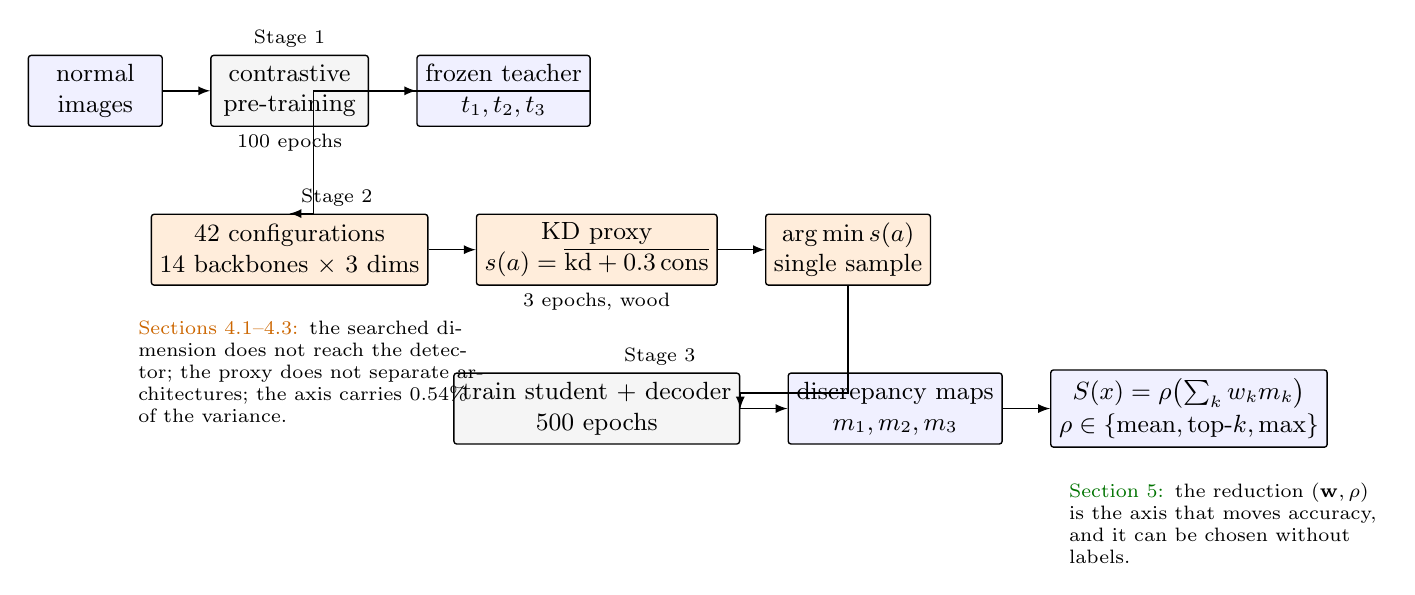
\begin{tikzpicture}[
  font=\small,
  node distance=4mm,
  box/.style={draw, rounded corners=1pt, align=center, inner sep=3pt,
              minimum height=9mm, line width=0.5pt},
  stage/.style={box, fill=black!4, minimum width=20mm},
  data/.style={box, fill=blue!6, minimum width=17mm},
  sel/.style={box, fill=orange!14, minimum width=20mm},
  arr/.style={->, >=latex, line width=0.5pt},
  lab/.style={font=\scriptsize, inner sep=1pt},
]

%% ---------- Stage 1 ----------
\node[data] (imgs) {normal\\images};
\node[stage, right=6mm of imgs] (teacher) {contrastive\\pre-training};
\node[data, right=6mm of teacher] (frozen) {frozen teacher\\$t_1,t_2,t_3$};

\draw[arr] (imgs) -- (teacher);
\draw[arr] (teacher) -- (frozen);
\node[lab, above=0.5mm of teacher] {Stage 1};
\node[lab, below=0.5mm of teacher] {100 epochs};

%% ---------- Stage 2 ----------
\node[sel, below=11mm of teacher] (space) {42 configurations\\14 backbones $\times$ 3 dims};
\node[sel, right=6mm of space] (proxy) {KD proxy\\$s(a)=\overline{\mathrm{kd}+0.3\,\mathrm{cons}}$};
\node[sel, right=6mm of proxy] (argmin) {$\arg\min s(a)$\\single sample};

\draw[arr] (space) -- (proxy);
\draw[arr] (proxy) -- (argmin);
\node[lab, below=0.5mm of proxy] {3 epochs, wood};
\node[lab, above=0.5mm of space, xshift=6mm] {Stage 2};

%% ---------- Stage 3 ----------
\node[stage, below=11mm of proxy] (rd) {train student $+$ decoder\\500 epochs};
\node[data, right=6mm of rd, minimum width=23mm] (maps) {discrepancy maps\\$m_1,m_2,m_3$};

\draw[arr] (rd) -- (maps);
\node[lab, above=0.5mm of rd, xshift=8mm] {Stage 3};

%% ---------- the scoring policy ----------
\node[data, right=6mm of maps] (pool) {$S(x)=\rho\!\left(\sum_k w_k m_k\right)$\\[1pt]
     $\rho\in\{\text{mean},\text{top-}k,\max\}$};

\draw[arr] (maps) -- (pool);

%% ---------- arrows between stages ----------
\draw[arr] (argmin.south) |- ([yshift=2mm]rd.east) -- (rd.east);
\draw[arr] (frozen.east) -| ([xshift=3mm]space.north) -- (space.north);

%% ---------- annotation: what the paper measures ----------
\node[lab, align=left, text width=44mm, anchor=north west]
  at ([xshift=-2mm,yshift=-4mm]space.south west) {%
  \textcolor{orange!80!black}{Sections 4.1--4.3:} the searched dimension does not
  reach the detector; the proxy does not separate architectures; the axis carries
  $0.54\%$ of the variance.};

\node[lab, align=left, text width=40mm, anchor=north west]
  at ([xshift=2mm,yshift=-4mm]pool.south west) {%
  \textcolor{green!45!black}{Section 5:} the reduction $(\mathbf{w},\rho)$ is the
  axis that moves accuracy, and it can be chosen without labels.};

\end{tikzpicture}
}
\caption{The pipeline under study. A teacher is pre-trained on normal images
(Stage~1); an architecture is selected from 42 configurations by minimising a
short-training distillation proxy on one category (Stage~2); the selected
architecture is then trained as a reverse-distillation detector (Stage~3) and each
test image is scored by reducing its multi-scale discrepancy maps with a policy
$(\mathbf{w},\rho)$. This paper measures the two axes in bold: the architecture
that Stage~2 selects, and the reduction that Stage~3 applies.}
\label{fig:pipeline}
\end{figure*}


Two teachers exist in this pipeline and they are not the same network. For the
search signal of Stage~2, a ResNet-18 teacher with a 128-dimensional projection
head is pre-trained for 100 epochs on the normal training images of the search
category
with a contrastive objective, and frozen thereafter; its role is to define the
feature space that the proxy score compares against. The \emph{deployed} detector
of Stage~3, however, builds its teacher from
ImageNet-1k weights~\cite{deng2022reverse,he2016deep}: the
\texttt{TeacherFeatureExtractor} instantiates a ResNet-18 initialised from
\texttt{ResNet18\_Weights.IMAGENET1K\_V1}, freezes it, and never adapts it to the
category being inspected. The two roles are worth separating explicitly. Every
detection result reported in this paper --- the variance decomposition of
Section~\ref{sec:diagnosis}, the policy comparison of Section~\ref{sec:leverage},
and the positioning of Section~\ref{sec:positioning} --- is produced by the
\emph{deployed} detector, and therefore rests on the ImageNet teacher; the
contrastive teacher never scores an image for reporting and enters only through the
Stage-2 proxy. The ImageNet teacher is a deviation from the reverse-distillation
recipe, which pre-trains the teacher on the target category's normal images
without labels; we report it here rather than leave it implicit, and
Section~\ref{subsec:resolvability} treats it as one candidate explanation for the
gap to the published numbers of Section~\ref{sec:positioning}.

Whichever teacher is in use contributes intermediate features at three
resolutions: the outputs of \texttt{layer1}, \texttt{layer2} and \texttt{layer3},
of shape $64\times56\times56$, $128\times28\times28$ and $256\times14\times14$ for
an input resized to $224\times224$.

\subsection{Stage 2: Architecture Search}
\label{subsec:nas}

The search space is the Cartesian product of 14 backbones and three feature
dimensions, giving 42 configurations. The backbones span convolutional and
attention-based families from 2015 to 2023, including
ResNets~\cite{he2016deep}, EfficientNet variants, MobileNetV3 and MobileOne, ViT
and DeiT variants, Swin-Tiny, and the ConvNeXt and ConvNeXt~V2
families~\cite{woo2023convnextv2}; Section~\ref{sec:positioning} lists them with
their deployed sizes. The three feature dimensions are 128, 256 and 512.

\subsubsection*{The evaluation signal}
Each candidate is evaluated by building a student with the candidate's backbone
and projection dimension, training it for a small number of epochs on the normal
training images of the search category, and then measuring a composite
distillation loss over validation batches $\mathcal{B}$ of held-out normal images:
%
\begin{equation}
\label{eq:proxy}
s(a) \;=\; \frac{\sum_{b \in \mathcal{B}} \mathbb{1}\!\left[\ell(b) < \tau\right]\,\ell(b)}
{\max\!\left(\sum_{b \in \mathcal{B}} \mathbb{1}\!\left[\ell(b) < \tau\right],\, 1\right)},
\qquad
\ell(b) \;=\; \mathcal{L}_{\mathrm{kd}}(b) + 0.3\,\mathcal{L}_{\mathrm{cons}}(b),
\end{equation}
%
where $\mathcal{L}_{\mathrm{kd}}$ is the mean-squared error between the student's
projection and the teacher's, and $\mathcal{L}_{\mathrm{cons}}$ is the
mean-squared error between the student's projections of two independently
augmented views of the same batch. A validation batch is accumulated only if its
loss is finite and below a fixed threshold $\tau = 1000$; otherwise it is skipped
and does not enter either the numerator or the denominator. Lower is better. Each
trial constructs and trains a fresh student, and the protocol draws $100$ trials
from a space of only $42$ cells, so a cell is generally visited more than once and
each visit re-trains a stochastically initialised student. Repeated visits therefore
do give several independent scores for some cells; the search entry point, however,
returns only the winning architecture, so the value it reports carries no variance
estimate. The variance of the signal is estimated
separately, from the repeated-evaluation study of
Section~\ref{subsec:proxy_stability}.
The two numerical consequences of the indicator in
Equation~\eqref{eq:proxy} are examined in
Section~\ref{subsec:proxy_stability} and are stated here for completeness. If every
batch of a trial is skipped the denominator is $\max(0,1) = 1$ and the signal
returns exactly zero, which is the minimum of the range of $s$. And because a
skipped batch is excluded rather than counted, the returned value is the mean over
the batches that survived, not over the batches that were drawn. Because the
backbones produce features of different
dimensionality while the teacher projects into a 128-dimensional space, a
candidate whose projection dimension differs from 128 is additionally given a
learned linear layer that maps the student's output into the teacher's space
before the losses are computed; this alignment layer exists only during search.

The search draws candidates uniformly at random from the 42 cells and returns the
one with the smallest score,
%
\begin{equation}
\label{eq:argmin}
a^\star \;=\; \arg\min_{a \in \mathcal{A}_{\text{sampled}}} \; s(a),
\end{equation}
%
and the number of draws is a protocol parameter (the recorded runs used 100, of
which a variable number complete successfully).

\subsection{Stage 3: Reverse-Distillation Detection}
\label{subsec:rd_detection}

The selected configuration is re-instantiated as a detector. A student encoder
takes the backbone's final feature map, adaptively pools it to $14\times14$, and
projects it through a $1\times1$ convolution with batch normalisation and ReLU to
a bottleneck of width $B$. A decoder then reconstructs the teacher's features in
reverse order: a first block produces the $14\times14$ stage at 256 channels, the
output is upsampled and passed through a second block producing the $28\times28$
stage at 128 channels, and upsampled again through a third block producing the
$56\times56$ stage at 64 channels. We note for later use that the bottleneck width
is fixed at $B = 256$ in the deployment path, independently of the feature
dimension that the search may have selected;
Section~\ref{subsec:inert} shows that this makes the searched dimension
unobservable in the deployed detector. The detector is trained on the normal
training images of each category separately, with AdamW at a learning rate of
$10^{-3}$ and weight decay $10^{-4}$, a cosine schedule, and random horizontal
flipping with probability $0.5$; the loss is the sum of mean-squared errors
between the student's reconstructions and the teacher's features at the three
scales.

\subsubsection*{Anomaly scoring}
\label{subsubsec:scoring}
Given a test image $x$, the teacher produces features $t_1, t_2, t_3$ and the
student produces reconstructions $s_1, s_2, s_3$. For each scale $k$ we form a
discrepancy map
%
\begin{equation}
\label{eq:diffmap}
m_k(x) \;=\; \bigl\| s_k(x) - t_k(x) \bigr\|_2 ,
\end{equation}
%
taking the $L_2$ norm across channels, and upsample each map to the input
resolution. An image-level score is then obtained by combining the maps with
non-negative weights $\mathbf{w} = (w_1, w_2, w_3)$ on the probability simplex and
reducing the resulting map to a scalar with a pooling operator $\rho$:
%
\begin{equation}
\label{eq:policy}
\begin{aligned}
S(x) &\;=\; \rho\!\left( \textstyle\sum_{k} w_k \, m_k(x) \right), \\
\rho &\in \{\,\text{mean},\ \text{top-}k,\ \max\,\}.
\end{aligned}
\end{equation}
%
We refer to the pair $(\mathbf{w}, \rho)$ as the \emph{scoring policy}. The
published pipeline uses $\mathbf{w} = (\tfrac13,\tfrac13,\tfrac13)$ and
$\rho = \text{mean}$, that is, an unweighted average over all pixels of the sum of
the three maps. This choice is not forced by the method: given a trained detector
the maps $m_k$ are already computed, so any policy can be evaluated on the same
model. Section~\ref{sec:leverage} evaluates a fixed grid of policies drawn from
Equation~\eqref{eq:policy}; we do not anticipate its result here, except to note
that the policy is a design choice the search does not touch.
\subsection{Protocol and Implementation Details}
\label{subsec:implementation}

Unless stated otherwise, the detector above is trained for 500 epochs with batch
size 64 and seed 42, with a ResNet-18 teacher, on the MVTec-AD
dataset~\cite{bergmann2021mvtec}. The search uses three quick training epochs per
candidate with batch size 16 on the \texttt{wood} category. Each search run
performs 100 draws from the 42-cell space (Section~\ref{subsec:proxy_stability});
the recorded runs used 100, of which a variable number completed. Inputs are resized to $224\times224$ and normalised with ImageNet
statistics. All figures report image-level AUROC averaged over the 15 categories.
Where a backbone's memory footprint exceeds the device at batch size 64, training
uses gradient accumulation with a smaller micro-batch, keeping the effective batch
size at 64; the micro-batch used is recorded per run and this affects only the
largest backbones.

\subsection{Use of Generative AI in This Work}
\label{subsec:genai}

In accordance with the journal's disclosure requirement, we state the role of
generative AI explicitly rather than only in the back matter. An AI assistant (a
large language model) was used substantially. It wrote the code for the diagnostic
experiments, the synthetic reproduction and the benchmark harness; it executed
those experiments and produced the numerical results reported here; and it
produced drafts of the manuscript text. It did not
determine the research questions, the experimental design or the interpretation of
the results. The authors specified the research questions, directed the work,
verified every reported result against the recorded experimental outputs, and take
full responsibility for the content, the claims and their accuracy. No figure or
table in this paper was generated by a generative model. Every figure is a direct
plot of recorded measurements, produced by the released script
\texttt{make\_figures\_v2.py} from the released JSON result files, and every table
is a transcription of the same files; the AI assistant wrote the plotting code and
ran it, but drew no image content and invented no data. All code, logs and derived
artefacts are released
so that every number can be traced to the run that produced it
(Section~\ref{sec:conclusion}).

% ============================================================================
% DRAFT v2 -- Section 4: Where the accuracy comes from (diagnosis)
% Every number here traces to:
%   search_forensics/search_forensics.json     (recorded runs)
%   proxy_diag/phaseA_proxy.json               (proxy repeatability, 420 calls)
%   proxy_diag/phaseB_truth.json               (210-detector truth matrix)
%   capacity_experiment/                       (parameter-capacity bands)
%   proxy_diag/samplesize_analysis.json        (resolvability, 4.4)
% ============================================================================

\section{Results: What the Architecture Search Actually Optimises}
\label{sec:diagnosis}

The three-stage pipeline of Section~\ref{sec:method} treats the Stage-2 search as
the component that produces the architecture, and the reported accuracy as
evidence that the search worked. This section tests that reading directly. We ask
four questions in turn: does the searched quantity reach the deployed model
(Section~\ref{subsec:inert}), is the search signal stable enough to be ranked
(Section~\ref{subsec:proxy_stability}), does the axis being searched have any
measurable effect on detection accuracy at all (Section~\ref{subsec:capacity_null}),
what does the search actually return when it is run
(Section~\ref{subsec:search_vs_random}), and --- the question that bounds all the
others --- how large a difference can the benchmark that judges this pipeline
resolve in the first place (Section~\ref{subsec:resolvability})?

\subsection{Two Thirds of the Search Space Cannot Reach the Deployed Model}
\label{subsec:inert}

The search space is
$\mathcal{A} = \mathcal{B} \times \mathcal{D}$ with
$|\mathcal{B}| = 14$ backbones and
$\mathcal{D} = \{128, 256, 512\}$ feature dimensions, giving 42 configurations.
The dimension enters the search through the student projector,
\texttt{ContrastiveModel(\allowbreak projection\_dim=\allowbreak feature\_dim)}, so the proxy score does
depend on it. It does not, however, reach the detector. In the deployment path the
student encoder builds its bottleneck with a hard-coded width,
\texttt{StudentEncoder.forward} calling
\texttt{\_init\_bottleneck(f.shape[1], 256, ...)}, while the decoder is
constructed with the requested width, \texttt{Decoder(bottleneck\_dim=\dots)}. The
final training entry point constructs the detector as
\texttt{RDDetector(student\_backbone=..., teacher\_arch=...)}, never passing
\texttt{bottleneck\_dim}; the argument therefore keeps its default of 256 for
every configuration.

Two consequences follow. For any configuration whose searched dimension is not
256 the two halves of the network disagree, so the discrepancy cannot be
activated by simply passing the argument --- the axis is unreachable by
construction rather than merely unused. And all three values of the searched
dimension produce the \emph{identical} deployed detector for a given backbone: the
42-configuration space contains only 14 distinct models, so the remaining 28
configurations are deployment-equivalent duplicates of them.

The recorded runs behave as this analysis predicts. Across four independent
searches on the same data and the same space, the selected backbone is
\texttt{efficientnet\_b0} every time, whereas the selected feature dimension
differs between runs:
%
\begin{center}
\resizebox{\columnwidth}{!}{%
\begin{tabular}{lccc}
\toprule
Run & Trials (declared / recorded) & Selected backbone & Selected dim \\
\midrule
\texttt{stage2}                                  & 30 / 17 & \texttt{efficientnet\_b0} & 128 \\
\texttt{stage2\_rtx3090}                         & 30 / 15 & \texttt{efficientnet\_b0} & 512 \\
\texttt{stage2\_rtx3090\_100trials}              & 100 / 39 & \texttt{efficientnet\_b0} & 256 \\
\texttt{stage2\_topjournal\_15backbones\_fixed}  & 100 / 93 & \texttt{efficientnet\_b0} & 256 \\
\bottomrule
\end{tabular}}

\end{center}
%
The stable part of the outcome is the part that matters for deployment; the
unstable part is precisely the part that cannot affect it. The search expends
two thirds of its ranking capacity on a variable with no deployment meaning, and
reports the winner of that sub-ranking as a discovered design choice.

A second observation from the same table: the number of trials recorded is
systematically below the number declared. The search loop catches exceptions and
\texttt{continue}s without appending a result, so failed trials vanish from the
record and from the denominator of any success statistic.

\subsection{The Proxy Carries Almost No Architecture Signal, and Collapses to Zero}
\label{subsec:proxy_stability}

The proxy is the average over validation batches of
$\mathrm{kd} + 0.3\,\mathrm{consistency}$, and the candidate with the
\emph{lowest} score is selected. Two properties of the scoring code matter.
A validation batch is accumulated only when \texttt{isfinite(score)} \emph{and}
\texttt{score < 1000}; a rejected batch is skipped with a warning. And the average
is formed as \texttt{total\_score / max(count, 1)}: if every batch in a trial is
rejected then \texttt{count} is zero, and the function returns exactly
\texttt{0.0} --- which, because the search minimises, is the best score attainable
anywhere in the space. A trial that failed to produce a usable number is thus
indistinguishable from a trial that produced the best possible number.

To measure how often this happens, and what the proxy does the rest of the time,
we call the search's own evaluation method (\texttt{evaluate\_architecture}) on
MVTec wood --- the category the search uses --- and repeat every one of the 42
configurations ten times with independent seeds. Table~\ref{tab:proxy_repeats}
gives the result, and Figure~\ref{fig:proxy_repeatability} the same data.

\begin{table}[t]
\centering
\caption{Proxy repeatability, condensed. The search's own evaluation method is
called ten times for each of the 42 configurations on MVTec wood (420
evaluations). ``Zero'' is the fraction of repeats returning exactly $0.0$; ``CV''
is the within-configuration coefficient of variation, pooled over each backbone's
three dimensions. The two collapse-prone backbones are shown individually; of the
remaining twelve not one degenerate trial occurred in any repeat. Eleven of those
twelve --- all but \texttt{efficientnet\_b0}, whose repeats are degenerate-free
but wide --- have pooled medians spanning $7.540$--$7.971$ with CV between
$2.2\%$ and $12.1\%$; \texttt{efficientnet\_b0} itself has a pooled CV of $74\%$.
Their per-backbone values are released with the code.}
\label{tab:proxy_repeats}
\resizebox{\columnwidth}{!}{%
\begin{tabular}{lrrrr}
\toprule
Backbone & Repeats & Zero (\%) & Median proxy & CV (\%) \\
\midrule
\texttt{efficientnet\_b1}        & 30 & \textbf{73} & \textbf{0.000} & 169.5 \\
\texttt{mobilenetv3\_small\_100} & 30 & \textbf{13} & 7.979 & 180.9 \\
\midrule
twelve well-behaved backbones (each) & 30 & 0 & 7.540--7.971 & 2.2--74.0 \\
\midrule
\textbf{all 42 configurations}   & \textbf{420} & \textbf{6.2} & --- & --- \\
\bottomrule
\end{tabular}}

\end{table}

Two regimes appear, and both matter. Twelve of the fourteen backbones are well
behaved in the sense that matters for the search: not a single degenerate trial
occurred in any repeat, so $\argmin$ never returns the spurious optimum. Within
those twelve, eleven have within-configuration coefficients of variation between
$2.2\%$ and $12.1\%$; the twelfth, \texttt{efficientnet\_b0}, is degenerate-free
but noisy, with a pooled CV of $74\%$. Its median proxy ($12.1$) is also the
outlier of the group, which is why we report the span of the eleven. Two backbones
are broken, and severely so: \texttt{efficientnet\_b1} returns exactly $0.0$ in
$73\%$ of evaluations at every dimension, and \texttt{mobilenetv3\_small\_100} in
$13\%$. Across all 420 evaluations, 26 ($6.2\%$) returned exactly zero. The cause
is visible in the engine's own diagnostics --- the student diverges, and every
validation batch then trips the hard threshold:

\begin{quote}
\texttt{Warning: Invalid score detected (score=4.19e+28, kd=2.18e+28), skipping}
\end{quote}

\runinhead{The proxy does not distinguish architectures.}
\begin{figure}[t]
\centering
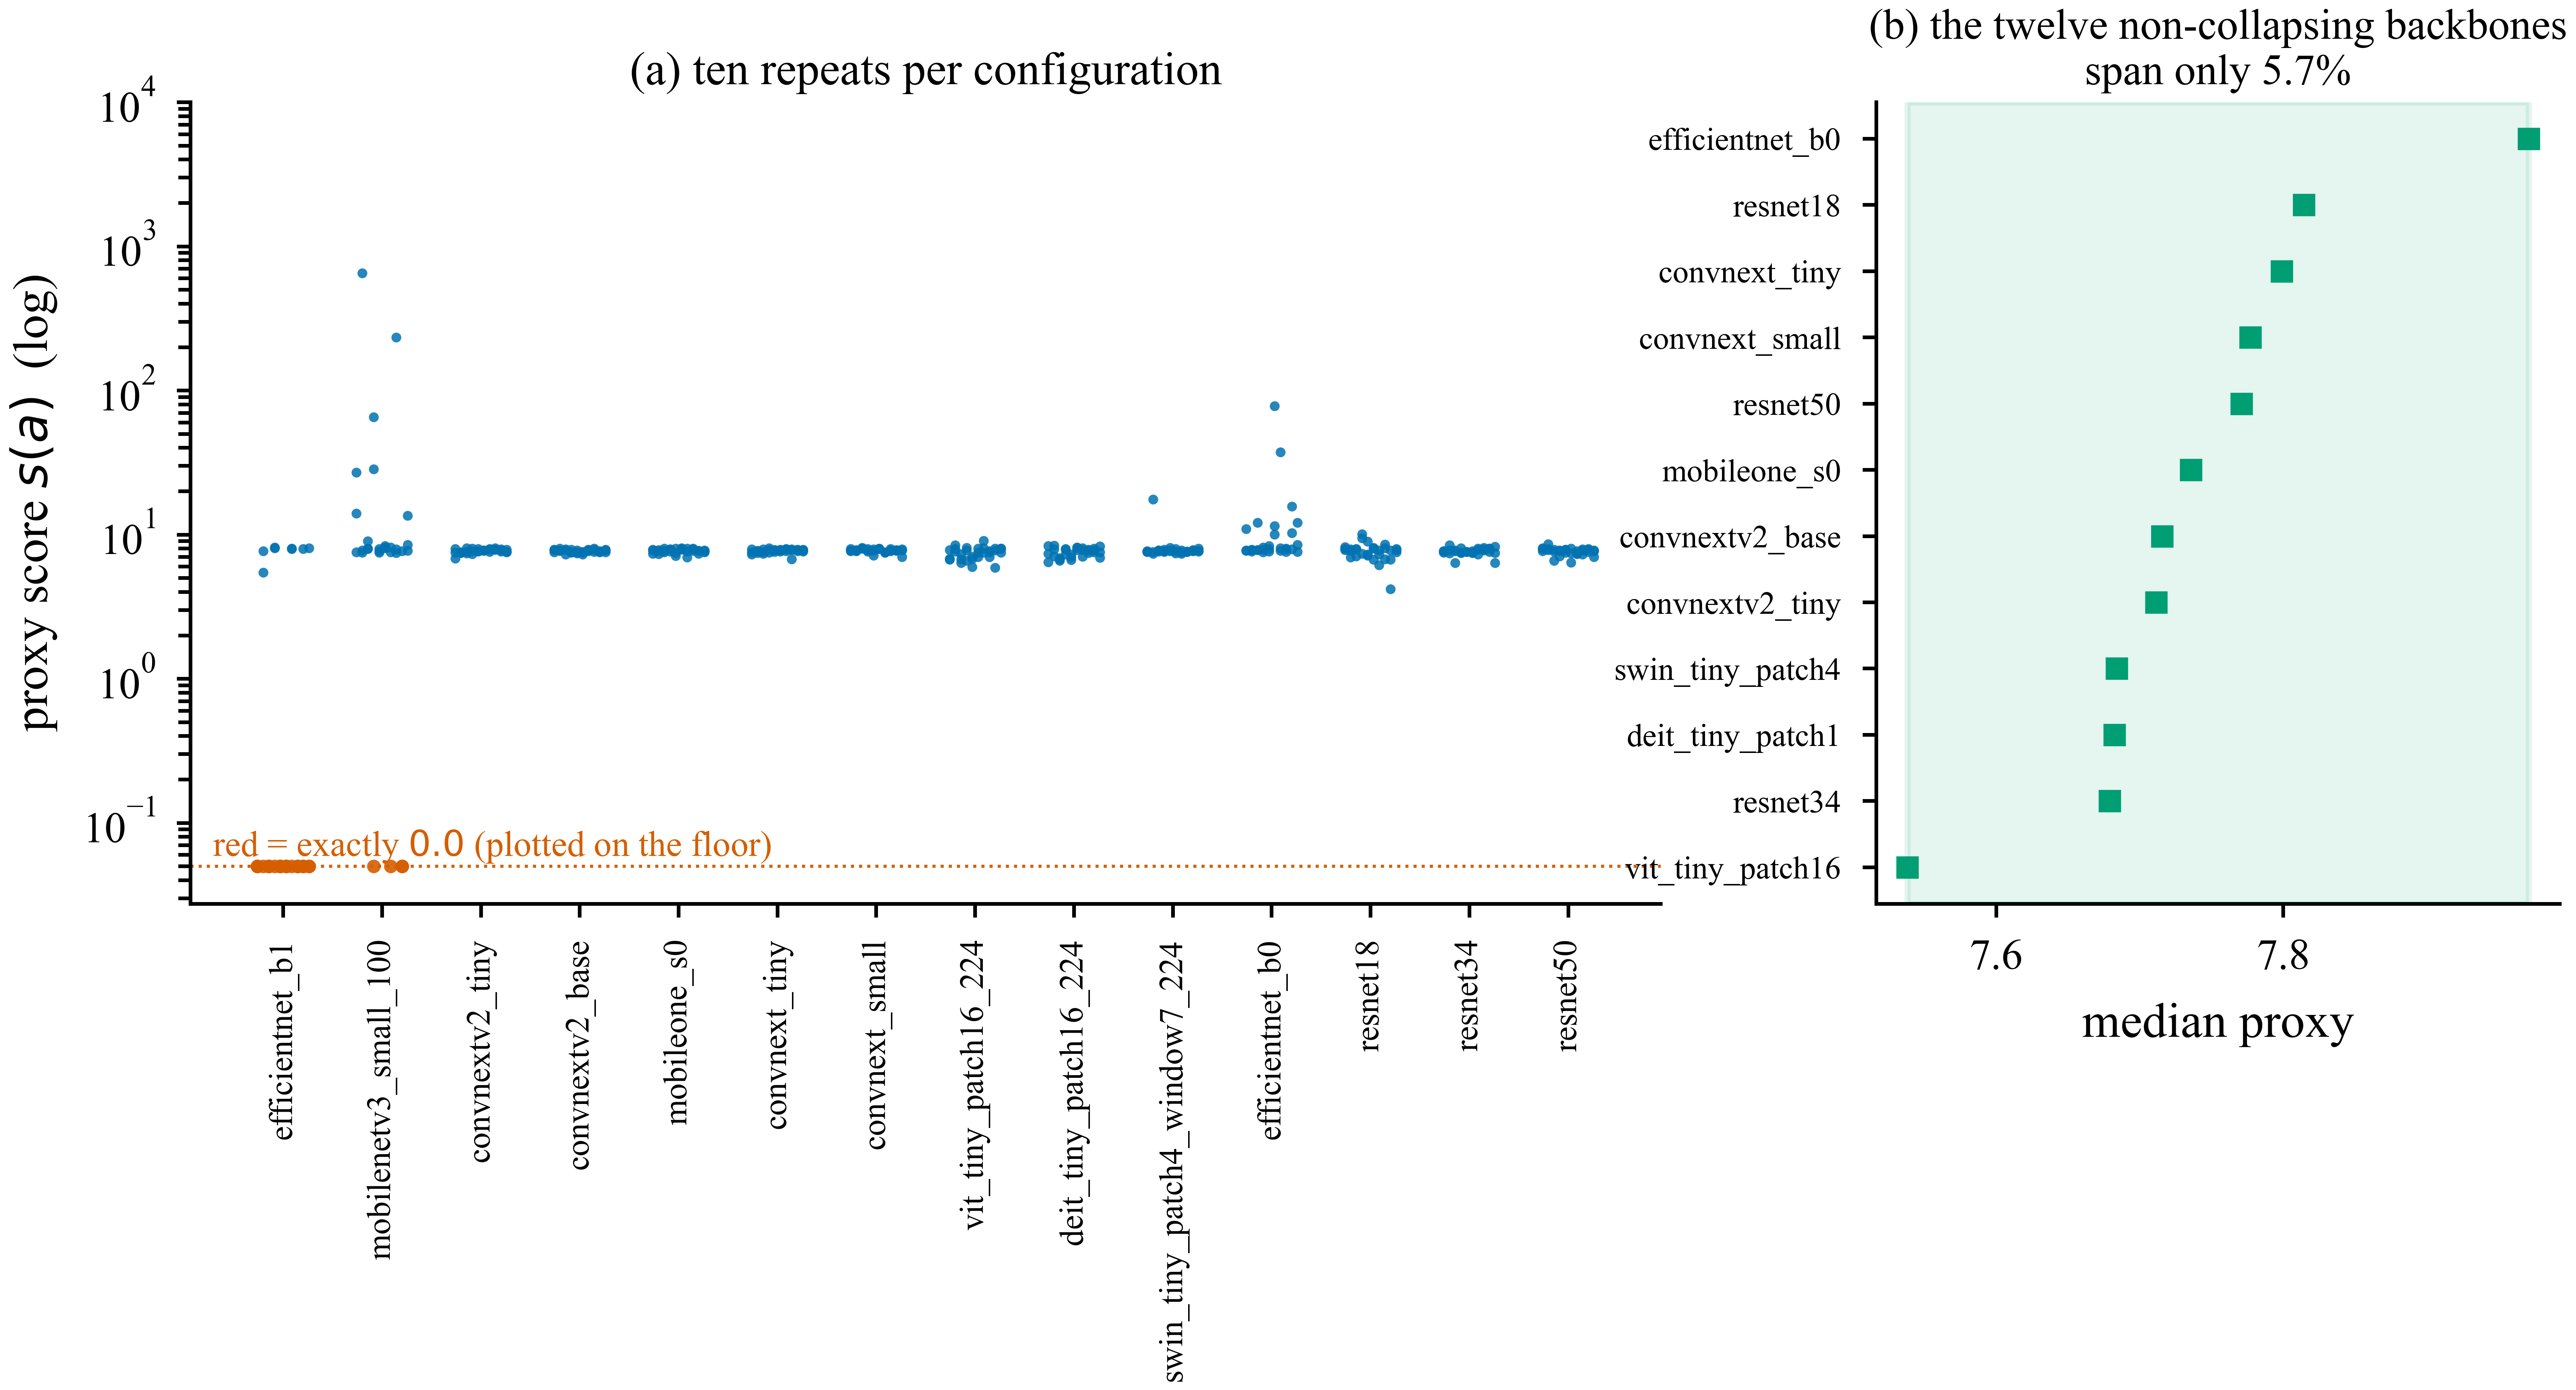
\includegraphics[width=\linewidth]{figures_v2/fig2_proxy_repeatability.png}
\caption{Proxy repeatability. (a) Ten independent evaluations of each of the 42
configurations, on a logarithmic axis. Eleven backbones form a tight band near
$7.6$ (\texttt{efficientnet\_b0} is degenerate-free but sits higher and wider);
\texttt{efficientnet\_b1} and \texttt{mobilenetv3\_small\_100} intermittently
return exactly $0.0$ (marked red, plotted on the axis floor) when their student
diverges. (b) The pooled median of the eleven tight non-collapsing backbones spans
only $5.7\%$, the same order as the within-configuration noise of a single
backbone.}
\label{fig:proxy_repeatability}
\end{figure}

The more consequential number in Table~\ref{tab:proxy_repeats} is the median
column. Across the eleven tight non-collapsing backbones --- CNN and Transformer
families, 2015-era through 2023-era, from ResNets~\cite{he2016deep} to ConvNeXt
V2~\cite{woo2023convnextv2} --- the median proxy spans only $7.54$ to $7.97$, a
range of $5.7\%$, while a single backbone's within-configuration noise is of the
same order ($2$--$12\%$ CV). The proxy contains essentially no
architecture-level signal. Any ranking it produces is not a ranking of
architectures; it is a ranking of which cell happened to be sampled.

\runinhead{Minimising then selects the broken cells.}
This turns a noisy score into a systematically wrong one. A well-behaved
configuration has a lower bound near $7.5$ and can never beat a configuration
that occasionally returns $0.0$. Minimising over the space does not select the
best candidate; it selects the candidate with the heaviest left tail --- and the
left tail is heaviest exactly where training diverged. Consistent with this,
\texttt{efficientnet\_b1}, the backbone that collapses in $73\%$ of evaluations,
is the $\argmin$ reported by the capacity searches of
Section~\ref{subsec:capacity_null} at two of their five parameter bands.

The recorded runs show the same pathology at the same rate. Over every search
result stored in the project --- 19 runs, 834 trials --- $8.0\%$ of trials score
exactly zero, and in \textbf{14 of the 19 runs (74\%)} the plain $\argmin$ over
the recorded results, which is literally what the search returns
(\texttt{min(self.results, key=score)}), points at a zero-score trial
(Table~\ref{tab:degeneracy}). The five capacity-budget searches are all affected,
and were usable only because a later analysis script discards trials scoring
$\le 0$: three different conventions for handling degenerate trials coexist in the
same codebase, the search engine keeping them while the downstream selectors drop
them.

\begin{table}[t]
\centering
\caption{Degenerate trials in the recorded searches, and whether the plain
$\argmin$ lands on one. A trial scoring exactly $0.0$ has had every validation
batch rejected, so the average is \texttt{total}/\texttt{max(count,1)}; because
the search minimises, such a trial wins outright.}
\label{tab:degeneracy}
\resizebox{\columnwidth}{!}{%
\begin{tabular}{lrrl}
\toprule
Run & Trials & Zeros & $\argmin$ config \\
\midrule
\texttt{cap\_budget\_3M}  & 20  & 1  & \texttt{mobilenetv3\_small\_100@128} \\
\texttt{cap\_budget\_6M}  & 40  & 4  & \texttt{mobilenetv3\_small\_100@256} \\
\texttt{cap\_budget\_8M}  & 80  & 11 & \texttt{efficientnet\_b1@256} \\
\texttt{cap\_budget\_13M} & 80  & 13 & \texttt{mobilenetv3\_small\_100@256} \\
\texttt{cap\_budget\_30M} & 80  & 6  & \texttt{efficientnet\_b1@256} \\
\texttt{mvtec\_stage2\_test/bottle} & 100 & 9 & \texttt{efficientnet\_b1@512} \\
\texttt{search\_strategies} (9 runs) & 270 & 23 & 8 of 9 degenerate \\
\midrule
\texttt{stage2} (main search) & 17 & 0 & \texttt{efficientnet\_b0@128} \\
\texttt{stage2\_rtx3090} & 15 & 0 & \texttt{efficientnet\_b0@512} \\
\texttt{stage2\_rtx3090\_100trials} & 39 & 0 & \texttt{efficientnet\_b0@256} \\
\texttt{stage2\_topjournal\_15backbones\_fixed} & 93 & 0 & \texttt{efficientnet\_b0@256} \\
\midrule
\textbf{Total} & \textbf{834} & \textbf{67 (8.0\%)} & \textbf{14 of 19 runs} \\
\bottomrule
\end{tabular}}

\end{table}

\runinhead{A reproducibility caveat.}
The recorded runs predate the current revision of the search engine, and the two
are not numerically identical: the recorded proxy for \texttt{efficientnet\_b0}
spans $0.002$--$0.065$, whereas the current code returns $7.5$--$12.2$ for the
same configuration. We therefore do not claim to reproduce the recorded search;
what the two lines of evidence agree on --- and all we rely on here --- is the
failure mode, its rate ($8.0\%$ against $6.2\%$) and the backbones it afflicts.
The revised engine also returns no zero-score trial in the four runs whose results
the manuscript reports, which is itself evidence of the revision; that the four
happened to select \texttt{efficientnet\_b0}, a backbone that does not collapse,
was in this account luck rather than method
(Section~\ref{subsec:search_vs_random}).

\runinhead{Two further obstacles.}
The proxy's absolute level is not comparable across categories: its median is
$0.110$ on \texttt{capsule}, $0.385$ on \texttt{hazelnut} and $7.56$ on
\texttt{wood}, a span of $68.6\times$, so neither a fixed threshold nor a
cross-category comparison of scores is meaningful --- yet the protocol runs a
single search on one category and transfers the winner to the others. And the
deployment-inert dimension of Section~\ref{subsec:inert}, which cannot change the
detector at all, nevertheless moves the proxy by a median factor of $1.16\times$
across 140 backbone comparisons and by more than $10\times$ at the 90th
percentile. A variable with no deployment meaning is responsible for
order-of-magnitude swings in the ranking.

\subsection{The Searched Axis Has No Measurable Effect on Accuracy}
\label{subsec:capacity_null}

A search that ranks noise could still be worth running if the axis it explores
mattered. We test that directly, by retraining detectors across the whole
parameter range under five mutually exclusive parameter bands, each trained with
the identical protocol (500 epochs, batch size 64, seed 42, ResNet-18 teacher,
reverse distillation). Within each band the search is restricted to backbones
whose deployed size (encoder plus decoder) falls inside the band, and the
best-scoring backbone is trained on all 15 MVTec-AD categories.
Table~\ref{tab:capacity_null} reports the result.

\begin{table}[t]
\centering
\caption{Parameter-capacity bands. Each band restricts the search to backbones
whose deployed size falls inside the band; the selected backbone is then trained
with the identical protocol on all 15 MVTec-AD categories.}
\label{tab:capacity_null}
\resizebox{\columnwidth}{!}{%
\begin{tabular}{llrr}
\toprule
Band & Selected backbone & Params (M) & Mean AUROC (\%) \\
\midrule
0--3M   & MobileNetV3-Small & 2.81  & 82.01 \\
3--6M   & EfficientNet-B0   & 5.41  & 83.14 \\
6--9M   & DeiT-Tiny         & 7.31  & 81.55 \\
9--15M  & ResNet-18         & 13.04 & \textbf{83.25} \\
15--31M & ResNet-50         & 25.77 & 83.08 \\
\bottomrule
\end{tabular}}

\end{table}

Multiplying the parameter budget by $9.2\times$ changes mean AUROC by
$+1.06$ percentage points, and the entire spread across the five bands is
$1.70$ points. The ordering is not monotone: the largest model is worse than the
second largest. All ten pairwise paired $t$-tests across categories are
non-significant (smallest $p = 0.058$).

We then measured the axis directly: all 14 backbones of the search space were
trained on all 15 MVTec-AD categories under the identical protocol, giving 210
detectors, and the resulting matrix was decomposed. A two-way decomposition
attributes \textbf{$0.54\%$} of the variance to the backbone
($F(13,182) = 1.844$, $p = 0.039$), \textbf{$95.32\%$} to the category, and
$4.13\%$ to their interaction, which is the error term in this repeated-measures
design (Figure~\ref{fig:variance}).

The backbone term is statistically significant: with 210 detectors the test has
the power to detect it. That, precisely, is the point. The effect is detectable
\emph{and} negligible. Architecture accounts for $0.54\%$ of the variance in
detection accuracy, against $95.32\%$ for which category is being inspected --- a
factor of $175$. A practitioner choosing between two backbones is moving an
AUROC whose variation is overwhelmingly determined by the object under
inspection rather than by the network.

The ranking says the same thing. Over the 15 categories the 14 backbones span
\begin{figure}[t]
\centering
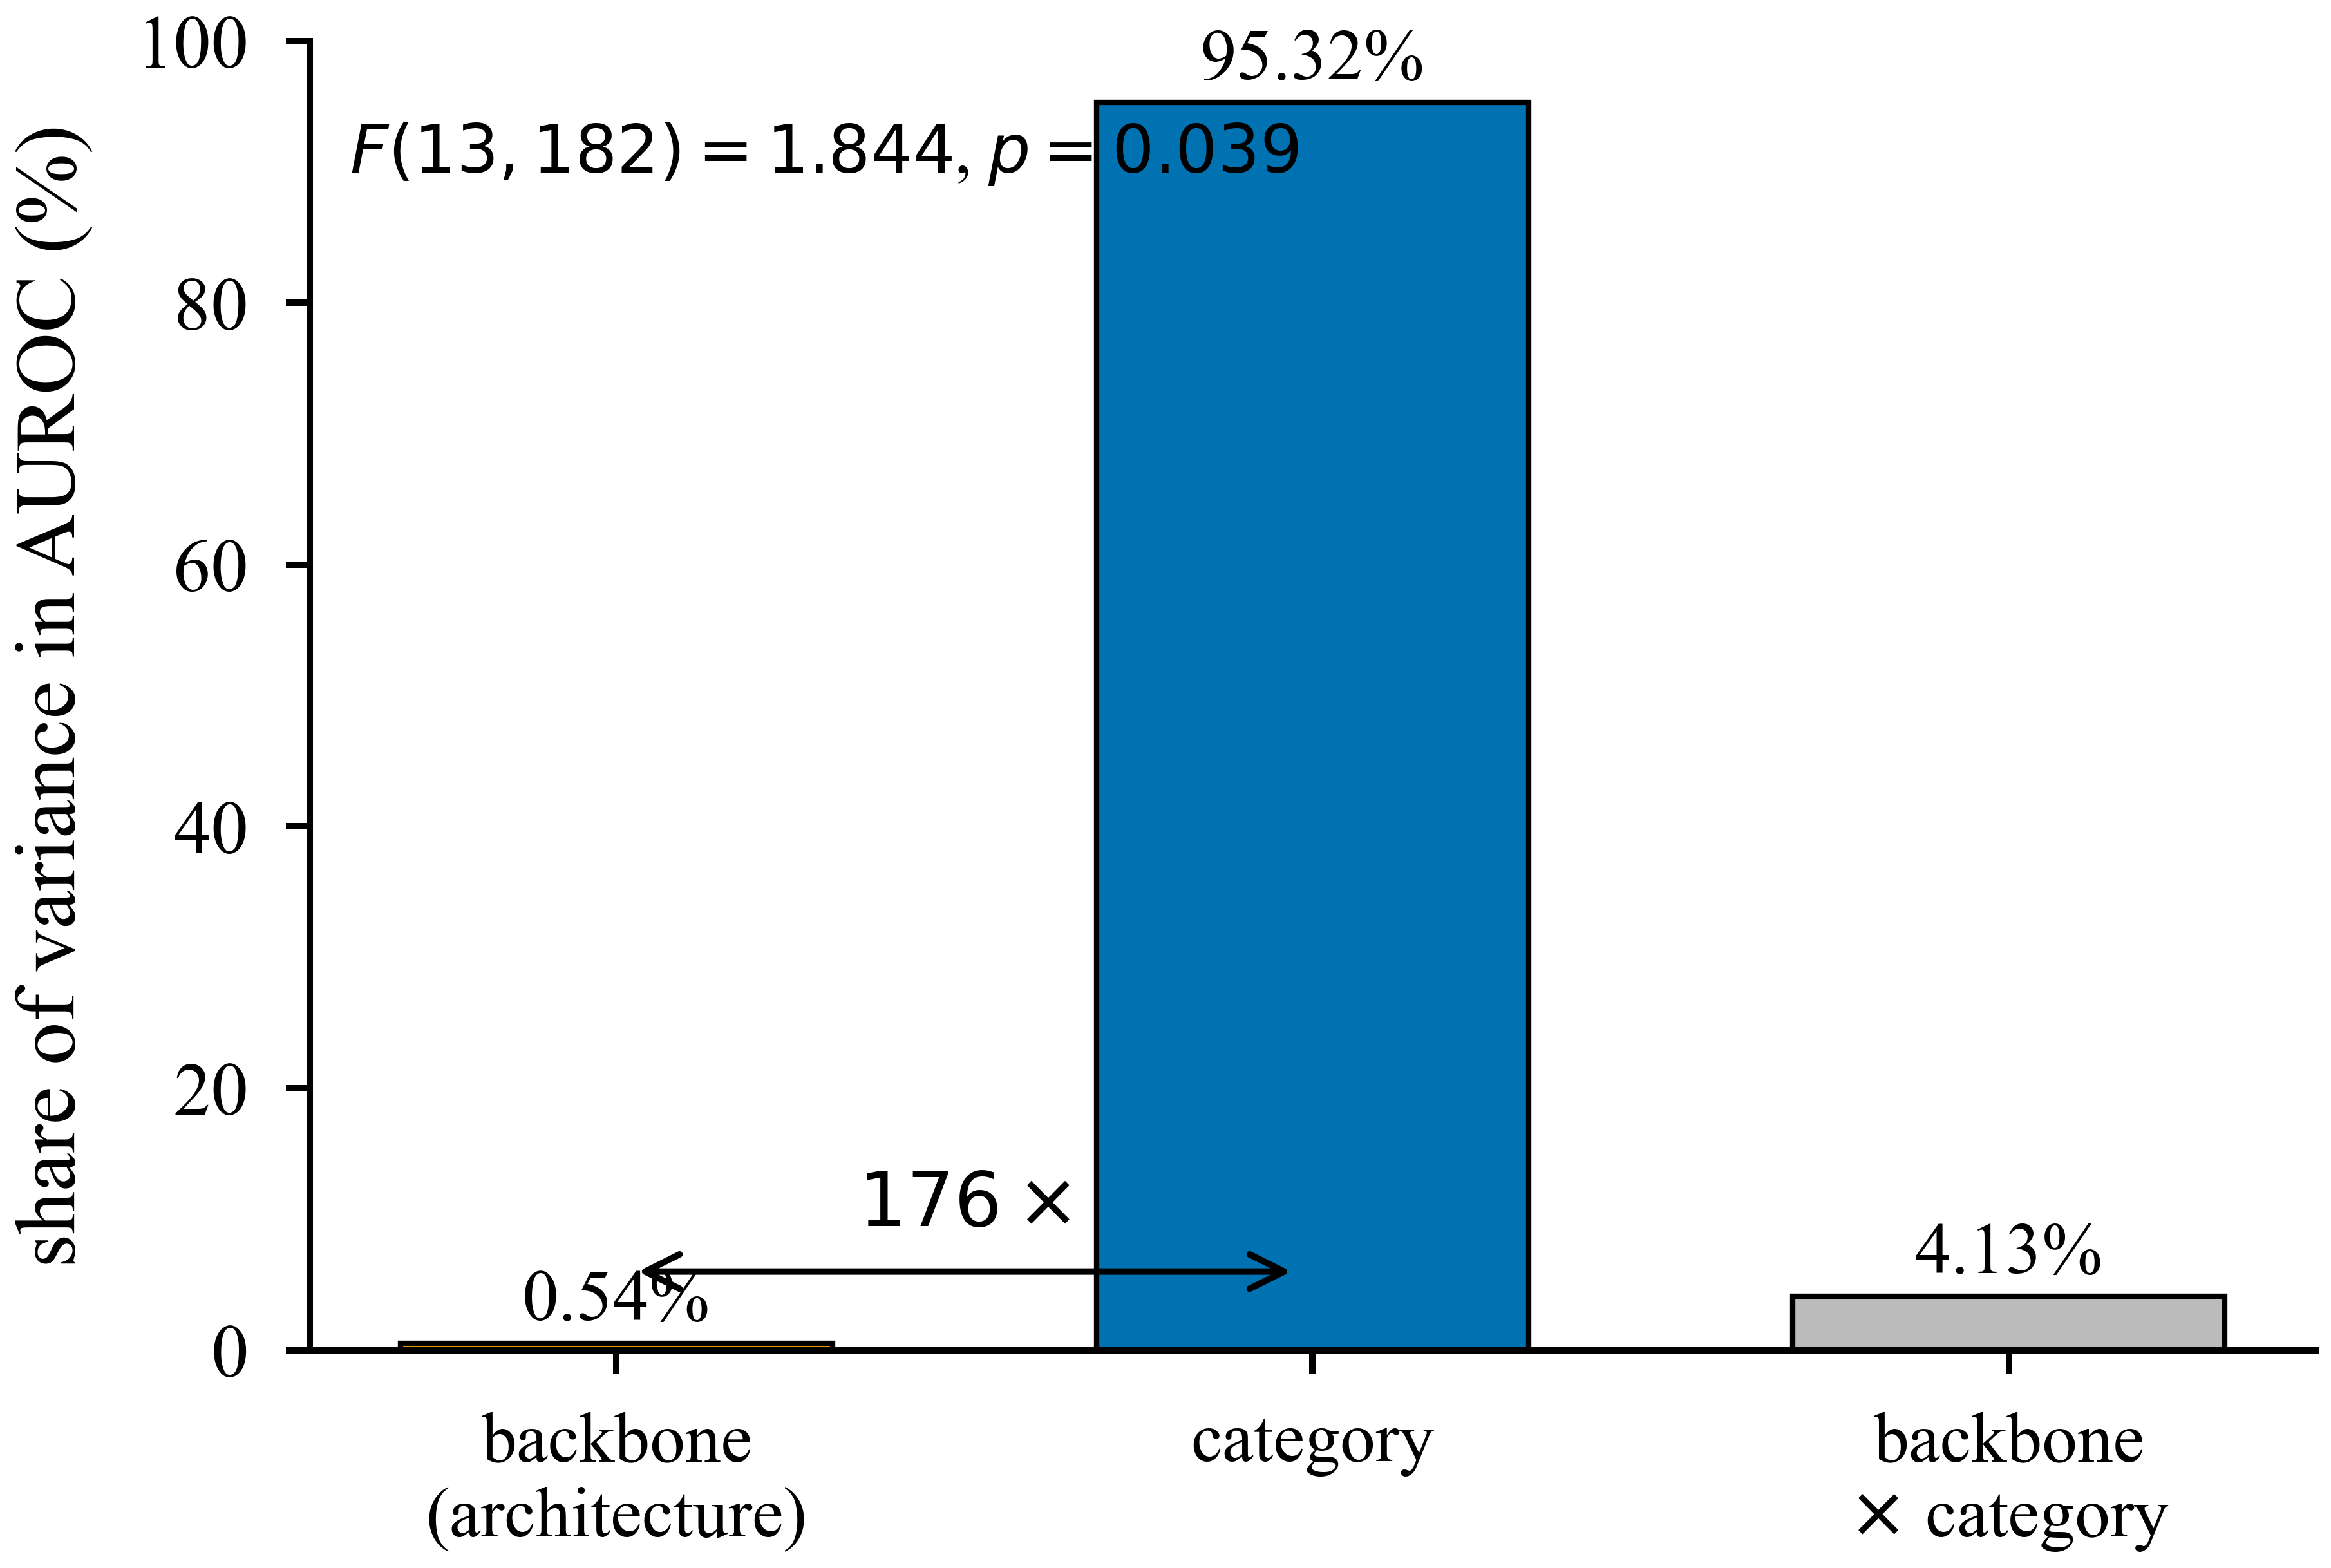
\includegraphics[width=\linewidth]{figures_v2/fig3_variance_decomposition.png}
\caption{Two-way decomposition of the true AUROC over 14 backbones and 15
categories (210 detectors). The backbone effect is statistically detectable and
practically negligible: it accounts for $0.54\%$ of the variance against $95.32\%$
for the category, a factor of $175$.}
\label{fig:variance}
\end{figure}

$3.98$ points of mean AUROC, and the eleven strongest span only $2.43$ points.
The manuscript's selected architecture, \texttt{efficientnet\_b0}, ranks fifth of
fourteen and is statistically indistinguishable from twelve of the thirteen
alternatives; only \texttt{convnextv2\_base} is significantly worse
($-3.11$ points, $p = 0.013$).

\runinhead{The search signal does not predict the target.}
Ranking the 14 backbones by their mean proxy score
(Section~\ref{subsec:proxy_stability}) and comparing that ordering with the true
performance matrix gives a Spearman correlation of \textbf{$-0.12$} ($p = 0.68$)
against the 15-category mean, and \textbf{$+0.02$} ($p = 0.93$) against
performance on \texttt{wood} itself. The search signal is not weakly correlated
with the outcome it exists to select for; on the very category the search is run
on it is indistinguishable from uncorrelated. The consequence is concrete: on
\texttt{wood} the backbone with the highest true AUROC is
\texttt{convnextv2\_base} at $94.74\%$, and across the fifteen categories
\texttt{convnextv2\_base} is the \emph{worst} of the fourteen at $79.36\%$; the
correlation between a backbone's rank on \texttt{wood} and its rank overall is
$-0.24$. The single category the protocol searches on is, if anything, mildly
anti-informative about the rest.

\runinhead{The run-to-run noise is not small.}
Within a fixed (backbone, category) cell the pooled standard deviation across
training seeds is $1.96$ points over 180 residual degrees of freedom, against a
total spread of $3.98$ points across the fourteen backbones. That the two numbers
are of the same order is the whole difficulty of this axis: a single training run
cannot resolve the backbone effect for any individual category, so a comparison
built on one run per configuration is unresolvable in principle rather than merely
imprecise. Section~\ref{subsec:resolvability} turns that into a number.

\runinhead{And the ranking does not transfer.}
Correlating the 14-backbone orderings of every pair of categories (105 pairs)
gives a mean Spearman $\rho = 0.215$, and in $31\%$ of pairs the two categories
\emph{disagree} on the ordering ($\rho < 0$). The protocol searches on a single
category, \texttt{wood}, and applies the winner to all fifteen. Since which
backbone is better depends on the category, a single-category search is not a
noisy estimate of a real quantity; it is an estimate of a quantity that does not
exist independently of the category.

This is the central observation of the paper. Taken with
Sections~\ref{subsec:inert} and~\ref{subsec:proxy_stability}, it says that the
proxy varies enormously across the space while the quantity it is supposed to
predict contributes half a percent of the variance that the category contributes
ninety-five percent of: the search ranks one noisy quantity in order to predict
another that is almost entirely determined by something else.

\subsection{What This Benchmark Design Can Resolve}
\label{subsec:resolvability}

The preceding subsections diagnose the search. This one asks a different
question, about the benchmark rather than about the pipeline: \emph{how small a
difference can the standard evaluation design detect?} The question is forced by
the state of the field. On MVTec-AD, PatchCore reached $99.1\%$ image-level
AUROC~\cite{roth2022patchcore} and the strongest methods reported since reach
$99.6\%$~\cite{liu2023simplenet,guo2025dinomaly}; the contested margin between
successive generations is $0.5$ points, on test sets holding roughly a hundred
images per category. If published comparisons cannot resolve differences of that
size, the ranking they produce is not a ranking of methods.

The 210-detector matrix of Section~\ref{subsec:capacity_null} and the replicated
cells within it supply every quantity the calculation needs. Three numbers come
out of them, all in AUROC points and all computed by
\texttt{proxy\_diag/samplesize\_analysis.py}:

\begin{itemize}
\item $\sigma_{\text{seed}} = 1.96$, the pooled within-cell standard deviation
over training seeds ($90$ cells replicated three times; $180$ residual degrees of
freedom). The distribution of per-cell standard deviations is heavily skewed ---
median $0.58$, maximum $7.74$ --- so the pooled figure is the honest single number
and the median understates the tail.
\item $\sigma_{\text{res}} = 3.30$, the two-way ANOVA residual on the single-seed
matrix. This is the working error for a comparison \emph{between} backbones,
because it also contains the backbone $\times$ category interaction that the
seed-only figure excludes.
\item $\sigma_{\Delta} = 4.12$, the empirical standard deviation of the
per-category difference between two backbones, averaged over the $91$ backbone
pairs. This is what a paired comparison across categories actually sees.
\end{itemize}

Two comparisons follow, and both are unfavourable to the design in common use. On
a \emph{single category}, with two backbones trained independently, the difference
has resolution $\sigma_{\text{seed}} = 1.96$ per arm; detecting the $0.5$-point
contested margin at $80\%$ power with a two-sided test at $\alpha = 0.05$ requires
\textbf{$240$ independent training runs per backbone}. Paired instead across the
fifteen categories the benchmark provides, the minimum detectable difference is
\textbf{$2.98$ points} --- $75\%$ of the entire $3.98$-point spread of the
fourteen backbones, and six times the margin the field argues about. Adding two
more training seeds per cell, as we do here, moves this only to $2.95$ points. To
resolve $0.5$ points by pairing over categories would take $532$ categories; the
benchmark has fifteen.

The requirement is also method-specific, which is a further reason it has to be
reported rather than assumed. Running the same calculation on a PatchCore-style
memory-bank detector, benchmarked through the harness released with this paper,
gives a seed standard deviation of $0.51$ points and a requirement of only $17$
runs per backbone --- a factor of $14$ below the reverse-distillation pipeline
studied here. No single number of runs is therefore sufficient in this field; the
figure belongs with the method it describes.

The implication is not that this benchmark is worthless, but that a
single-category, single-run comparison on it cannot support a claim at the
resolution the literature reports. A backbone ranking must either be averaged over
many categories --- which is what Table~\ref{tab:controlled} does, and why that
table needed $210$ detectors --- or be reported with an explicit statement of what
it can and cannot distinguish. This is also why the architecture effect, though
statistically detectable at $210$ detectors ($p = 0.039$), cannot be
\emph{ranked} reliably by any smaller design: the power that makes the effect
visible is the same power the field's usual single-category design lacks. We adopt
this discipline for the rest of the paper, making every backbone comparison on the
15-category mean and reporting differences smaller than about three points as
unresolved rather than as rankings.

\subsection{Running the Search Selects the Broken Backbones}
\label{subsec:search_vs_random}

The preceding subsections describe a search space that is two thirds inert, a
signal that does not discriminate between architectures and collapses to a score
of exactly zero for two of them, and a target quantity that architecture barely
moves. This subsection asks what they amount to in practice, by simply running the
search. We invoke the search engine's own entry point
(\texttt{NASSearchEngine.search}) with the manuscript's settings --- 100 trials,
three quick training epochs per candidate, uniform sampling from the 42 cells ---
and repeat it with twelve independent seeds. Because the searched feature
dimension cannot reach the detector (Section~\ref{subsec:inert}), the deployed
model depends only on the selected backbone, so the true quality of a run's output
can be read directly off the truth matrix of
Section~\ref{subsec:capacity_null}. Every run returned one of the two backbones
that collapse to zero: eight of the twelve returned \texttt{efficientnet\_b1}
(true rank 12 of 14, $80.43\%$ mean AUROC) and four returned
\texttt{mobilenetv3\_small\_100} (rank 7 of 14, $81.85\%$). None of the other
twelve backbones was ever selected, and only 2 of the 14 backbones and 6 of the 42
configurations appeared at all. Under uniform selection the probability of twelve
runs all landing inside that two-element subset is $7.2\times10^{-11}$. The search
does not merely fail to find a good architecture; it is reliably drawn to the two
configurations that break.

The consequence is quantitative, and it is not marginal
(Figure~\ref{fig:search_vs_random}). Averaged over the twelve
runs the search's output attains \textbf{80.91}\% mean AUROC. Picking a backbone
uniformly at random from the same space gives \textbf{81.65}\% (bootstrap
s.d.\ 0.32 points), and the best backbone in the space gives \textbf{83.34}\%.
The search result sits at the \textbf{1.2th percentile} of the random-selection
distribution --- it is worse than $98.8\%$ of uniform draws --- with a mean true
rank of $10.3$ of $14$ against $7.5$ for random, and it never once selected one of
the four strongest backbones. Replacing the search with a random number generator
would have improved the deployed detector; replacing it with the constant
\texttt{resnet18} would have improved it by $2.4$ points.

The mechanism is the one established in Section~\ref{subsec:proxy_stability}: a
well-behaved configuration is bounded below by roughly $7$--$8$, while the two
collapse-prone backbones return exactly $0.0$ whenever their student diverges, so
minimising a single sample per configuration selects the heaviest left tail in the
space --- and the heaviest left tails belong to the configurations that failed.
More trials make this more certain rather than less, because every additional
sample of a collapse-prone backbone is another chance to return the minimum of the
space. The exclusion is not perfectly clean: in the twelve recorded runs
\texttt{efficientnet\_b0} also returned exactly $0.0$ twice, in $2.5\%$ of its 79
trials, against $82\%$ of 72 for \texttt{efficientnet\_b1} and $22\%$ of 87 for
\texttt{mobilenetv3\_small\_100} in the same runs. The two extremes dominate the
minimum, but no backbone is immune, which is why the fix has to be a filter rather
than a blacklist. Our recommendation therefore follows from the mechanism rather
than from any single run: \textbf{a search whose objective can silently return the
optimum of its own range must filter degenerate evaluations before minimising, and
should report the distribution of its per-configuration scores rather than a
single minimum.}

\runinhead{Why the earlier searches looked successful.}
\begin{figure}[t]
\centering
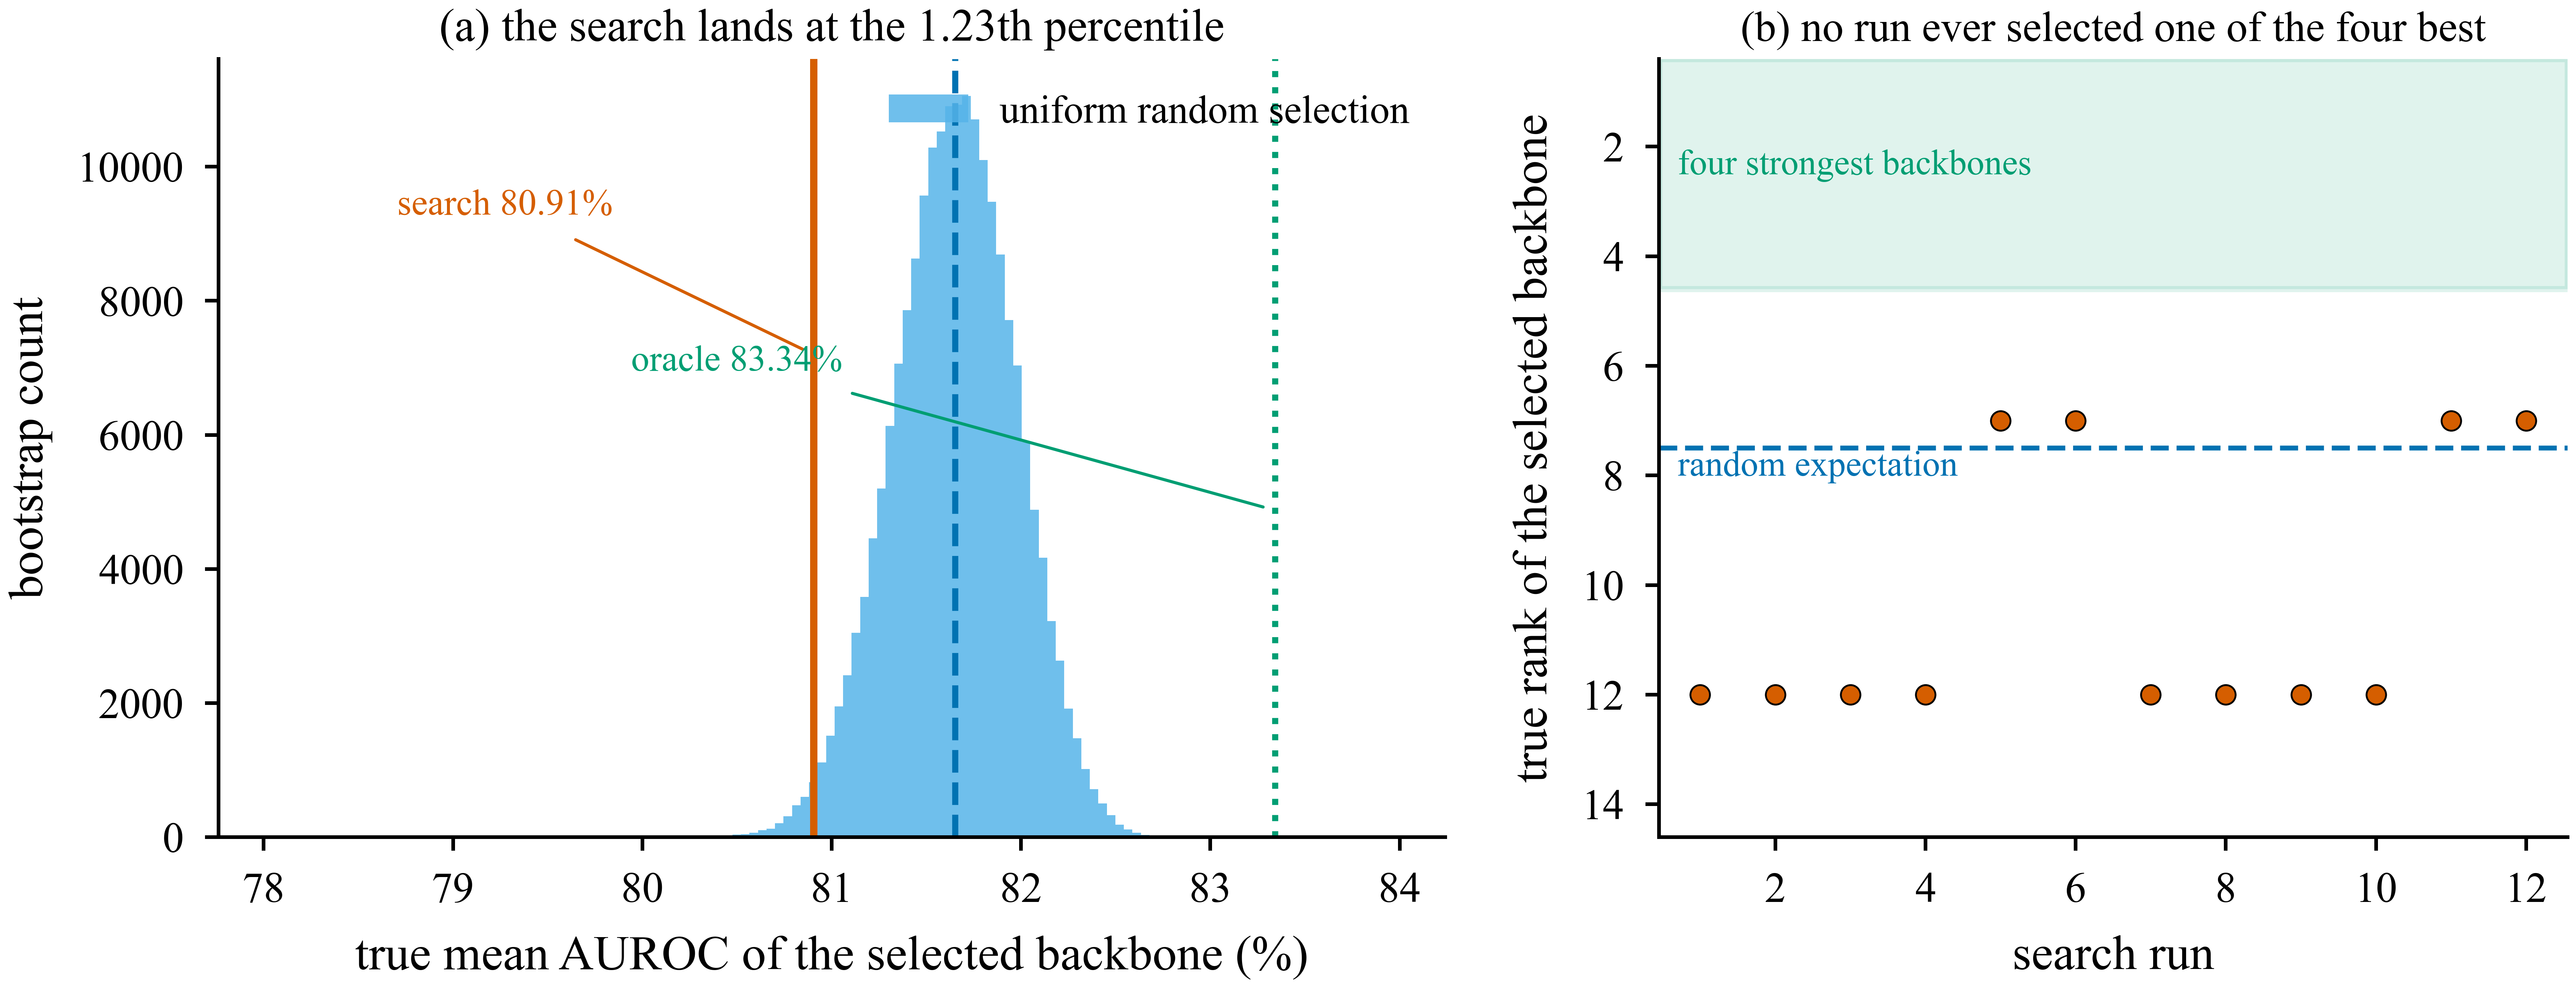
\includegraphics[width=\linewidth]{figures_v2/fig4_search_vs_random.png}
\caption{The search against chance. (a) Bootstrap distribution of the true mean
AUROC obtained by selecting a backbone uniformly at random from the same space,
with the search's output and the oracle marked. The search result sits at the
$1.2$th percentile. (b) True rank of the backbone returned by each of the twelve
runs: the four strongest backbones were never selected.}
\label{fig:search_vs_random}
\end{figure}

The four search runs whose results the manuscript reports selected
\texttt{efficientnet\_b0} (Section~\ref{subsec:inert}), a backbone that collapses
only rarely and never in those four runs. That this is luck rather than method is
the point of Section~\ref{subsec:search_vs_random}, and it is the reason we report
both lines of evidence rather than either alone.

% ============================================================================
% DRAFT v2 -- Section 5: Where the leverage actually is
% Numbers from fusion_policy/fusion_summary.json (E2), policy_select/ (E3),
% pseudo_select/ (E9, pending).
% ============================================================================

\section{Results: Where the Leverage Is --- the Inference-Time Scoring Policy}
\label{sec:leverage}

Section~\ref{sec:diagnosis} established that the design axis the pipeline
searches---the backbone---does not measurably move accuracy, while the search
signal used to choose within it is unstable. That raises an obvious question:
which design choices \emph{do} move accuracy? This section shows that the way
per-pixel discrepancies are combined into an image-level score---a choice that
requires no additional training to revisit---is worth an order of magnitude more
than the architecture.

\subsection{The Scoring Policy as a Design Axis}
\label{subsec:policy_space}

With a trained detector the anomaly score of an image is formed in two steps
(Section~\ref{subsec:rd_detection}): the discrepancy maps $m_1, m_2, m_3$ of the
three teacher scales are combined by non-negative weights, and the resulting map
is reduced to a scalar. The published pipeline fixes both choices implicitly:
uniform weights, and the arithmetic mean over all pixels.

Neither is forced by the method. We therefore treat the pair
$(\mathbf{w}, \rho)$ as a \emph{scoring policy}, with
$\mathbf{w}$ on the probability simplex over three scales and
$\rho \in \{\text{mean}, \text{top-}k, \text{max}\}$, where top-$k$ averages the
$k$ highest-scoring pixels with $k = 1\%$ of the map. We evaluate 82 policies:
the 66-point simplex grid at step $0.1$ crossed with top-$k$ pooling, plus 9
single-scale policies (\texttt{s1}, \texttt{s2}, \texttt{s3} $\times$ mean, top-$k$,
max), 3 policies that sum the three maps without weights, and 4 that normalise each
map before combining ($66+9+3+4 = 82$). The exact enumeration, with every
$(\mathbf{w},\rho)$ pair keyed by name, is released in
\texttt{fusion\_policy/fusion\_summary.json}.

A second and larger policy set is used in
Section~\ref{subsec:pseudo_results}, where the search over policies has to be
richer because the criterion rather than the pooling is under test: the finer
simplex grid at step $0.2$ is paired with all three reductions, and the coarser
step-$0.1$ grid is paired with top-$k$ pooling, together with the three canonical
uniform variants, giving $66 + 21 + 21 + 3 = 111$ policies. The two sets are not
interchangeable, and the numbers below are quoted per set; where they are compared
directly, Table~\ref{tab:ksweep} says so.

An important property of this axis is that a fixed grid of it can be evaluated
without retraining: changing $(\mathbf{w},\rho)$ requires no new parameters and no
extra inference, since the discrepancy maps are already computed and pooling is a
reduction over them, so every policy in the grid is evaluated on the \emph{same}
trained model. The simplex is continuous, so no finite grid can be exhaustive;
what we evaluate is a fixed grid of the size stated above, and the sensitivity
sweep of Section~\ref{subsec:policy_results} is what establishes that the grid is
fine enough for the conclusion. This is a practical convenience for deployment ---
the policy can be
re-tuned on an existing detector without repeating the training run --- and it is
what makes the grid evaluation below affordable.

It is worth being explicit that this does not diminish the role of training, and
we do not present the two axes as competing. Establishing that the architecture
axis is inert (Section~\ref{sec:diagnosis}) required retraining hundreds of
detectors, and we regard that expense as the necessary price of a defensible
claim. The axes are complementary: training determines what a model can
represent, and the scoring policy determines how much of that is read out.

\subsection{Exhaustive Evaluation on a Fixed Model}
\label{subsec:policy_results}

We train one detector per MVTec-AD category with the manuscript's protocol
(EfficientNet-B0 student, 500 epochs, batch size 64, seed 42, ResNet-18 teacher),
then evaluate all 82 policies on the frozen model. Table~\ref{tab:fusion} reports
the result.

\begin{table}[t]
\centering
\caption{Scoring policies evaluated on one frozen detector per category
(15 categories, 82 policies). ``Worst category'' is the lowest per-category
AUROC, i.e.\ the failure mode that matters in deployment. The default is the
policy the published pipeline uses. The per-category oracle \emph{reads the test
labels} to pick the best policy for each category and is an upper bound, not an
achievable result; every other row is label-free.}
\label{tab:fusion}
\resizebox{\columnwidth}{!}{%
\begin{tabular}{lrrr}
\toprule
Policy & Mean AUROC (\%) & Worst category (\%) & Extra retraining \\
\midrule
\texttt{mean}, uniform weights (default) & 82.80 & \textbf{42.22} & --- \\
\texttt{max}, uniform weights            & 86.84 & --- & none \\
\texttt{top-}k, uniform weights          & 90.21 & 78.37 & none \\
best single policy over the grid (\texttt{w0.3\_0.6\_0.1}, top-$k$; picked on
test, so also an oracle) & \textbf{90.60} & --- & none \\
\midrule
per-category oracle over 82 policies (uses labels)     & \textbf{93.72} & 84.67 & none \\
\bottomrule
\end{tabular}}

\end{table}

Switching the pooling from the arithmetic mean to top-$k$ raises mean AUROC from
$82.80\%$ to $90.21\%$, a gain of $7.42$ points, with no change to the model.
(Throughout this section the deltas are computed on the unrounded values and
rounded only for display, so a delta may differ by $0.01$ from the subtraction of
the two printed figures --- here $90.2075 - 82.7896 = 7.4179$.)
Scale weighting adds much less: the best weighted policy reaches $90.60\%$, only
$0.39$ points above the uniform top-$k$. Every one of the eight highest-scoring
policies uses top-$k$ pooling, and all of the improvement therefore comes from
the reduction step rather than from the scale weights. Choosing the policy
per category raises the mean further, to $93.72\%$---$10.92$ points above the
default, and again without retraining anything.

The pooling effect is not an artefact of one training run. Repeating the
comparison with two further seeds (43 and 44) gives $+8.07$ and $+7.78$ points
against $+7.42$ for the seed reported here; the per-seed estimates span
$0.65$ points. Aggregating the two later seeds alone gives policy means of
$82.36\%$ for the default and $90.28\%$ for top-$k$ ($+7.92$ points, seeds
$43$--$44$). We quote the per-seed estimates and that within-script aggregate
rather than one summary number, because seed~42's models enter the reported table
through a different evaluation script than the later two do
(Table~\ref{tab:ksweep}): averaging across the two scripts would average two
implementations of the same statistic, which we decline to do, so we do not quote a
single three-seed mean for this quantity.
Throughout, the seed reported in full is seed~42, on which the default and top-$k$
read $82.80\%$ and $90.21\%$ ($+7.42$); the headline we carry into the abstract
and conclusion is the conservative $+7.5$ points, the mean on the label-free
$70/30$ split of Section~\ref{subsec:pseudo_results}. Every quantity we can
measure for this effect therefore lies between $+7.4$ and $+8.1$ points, and we
quote the smallest of them as the headline.

\runinhead{The effect is not a hyper-parameter artefact.}
The comparison fixes $k = 1\%$ of the map, so it is fair to ask whether the gain
is an artefact of that choice. Sweeping $k$ over two orders of magnitude
(Table~\ref{tab:ksweep} and Figure~\ref{fig:ksweep}) traces a broad plateau rather than a spike: mean AUROC
rises from $86.74\%$ at $k = 1$ pixel to a maximum of $91.08\%$ at $k = 5\%$, and
stays above $89.6\%$ for every $k$ between $0.5\%$ and $20\%$. The default of
$1\%$ sits inside the plateau, not on its edge, and any value in that range
recovers $7$ to $8.4$ points. The worst-category statistic peaks earlier, at
$k = 2\%$ ($79.24\%$), so $k$ between $1\%$ and $2\%$ is the best compromise
between average accuracy and worst-case behaviour.

\begin{figure}[t]
\centering
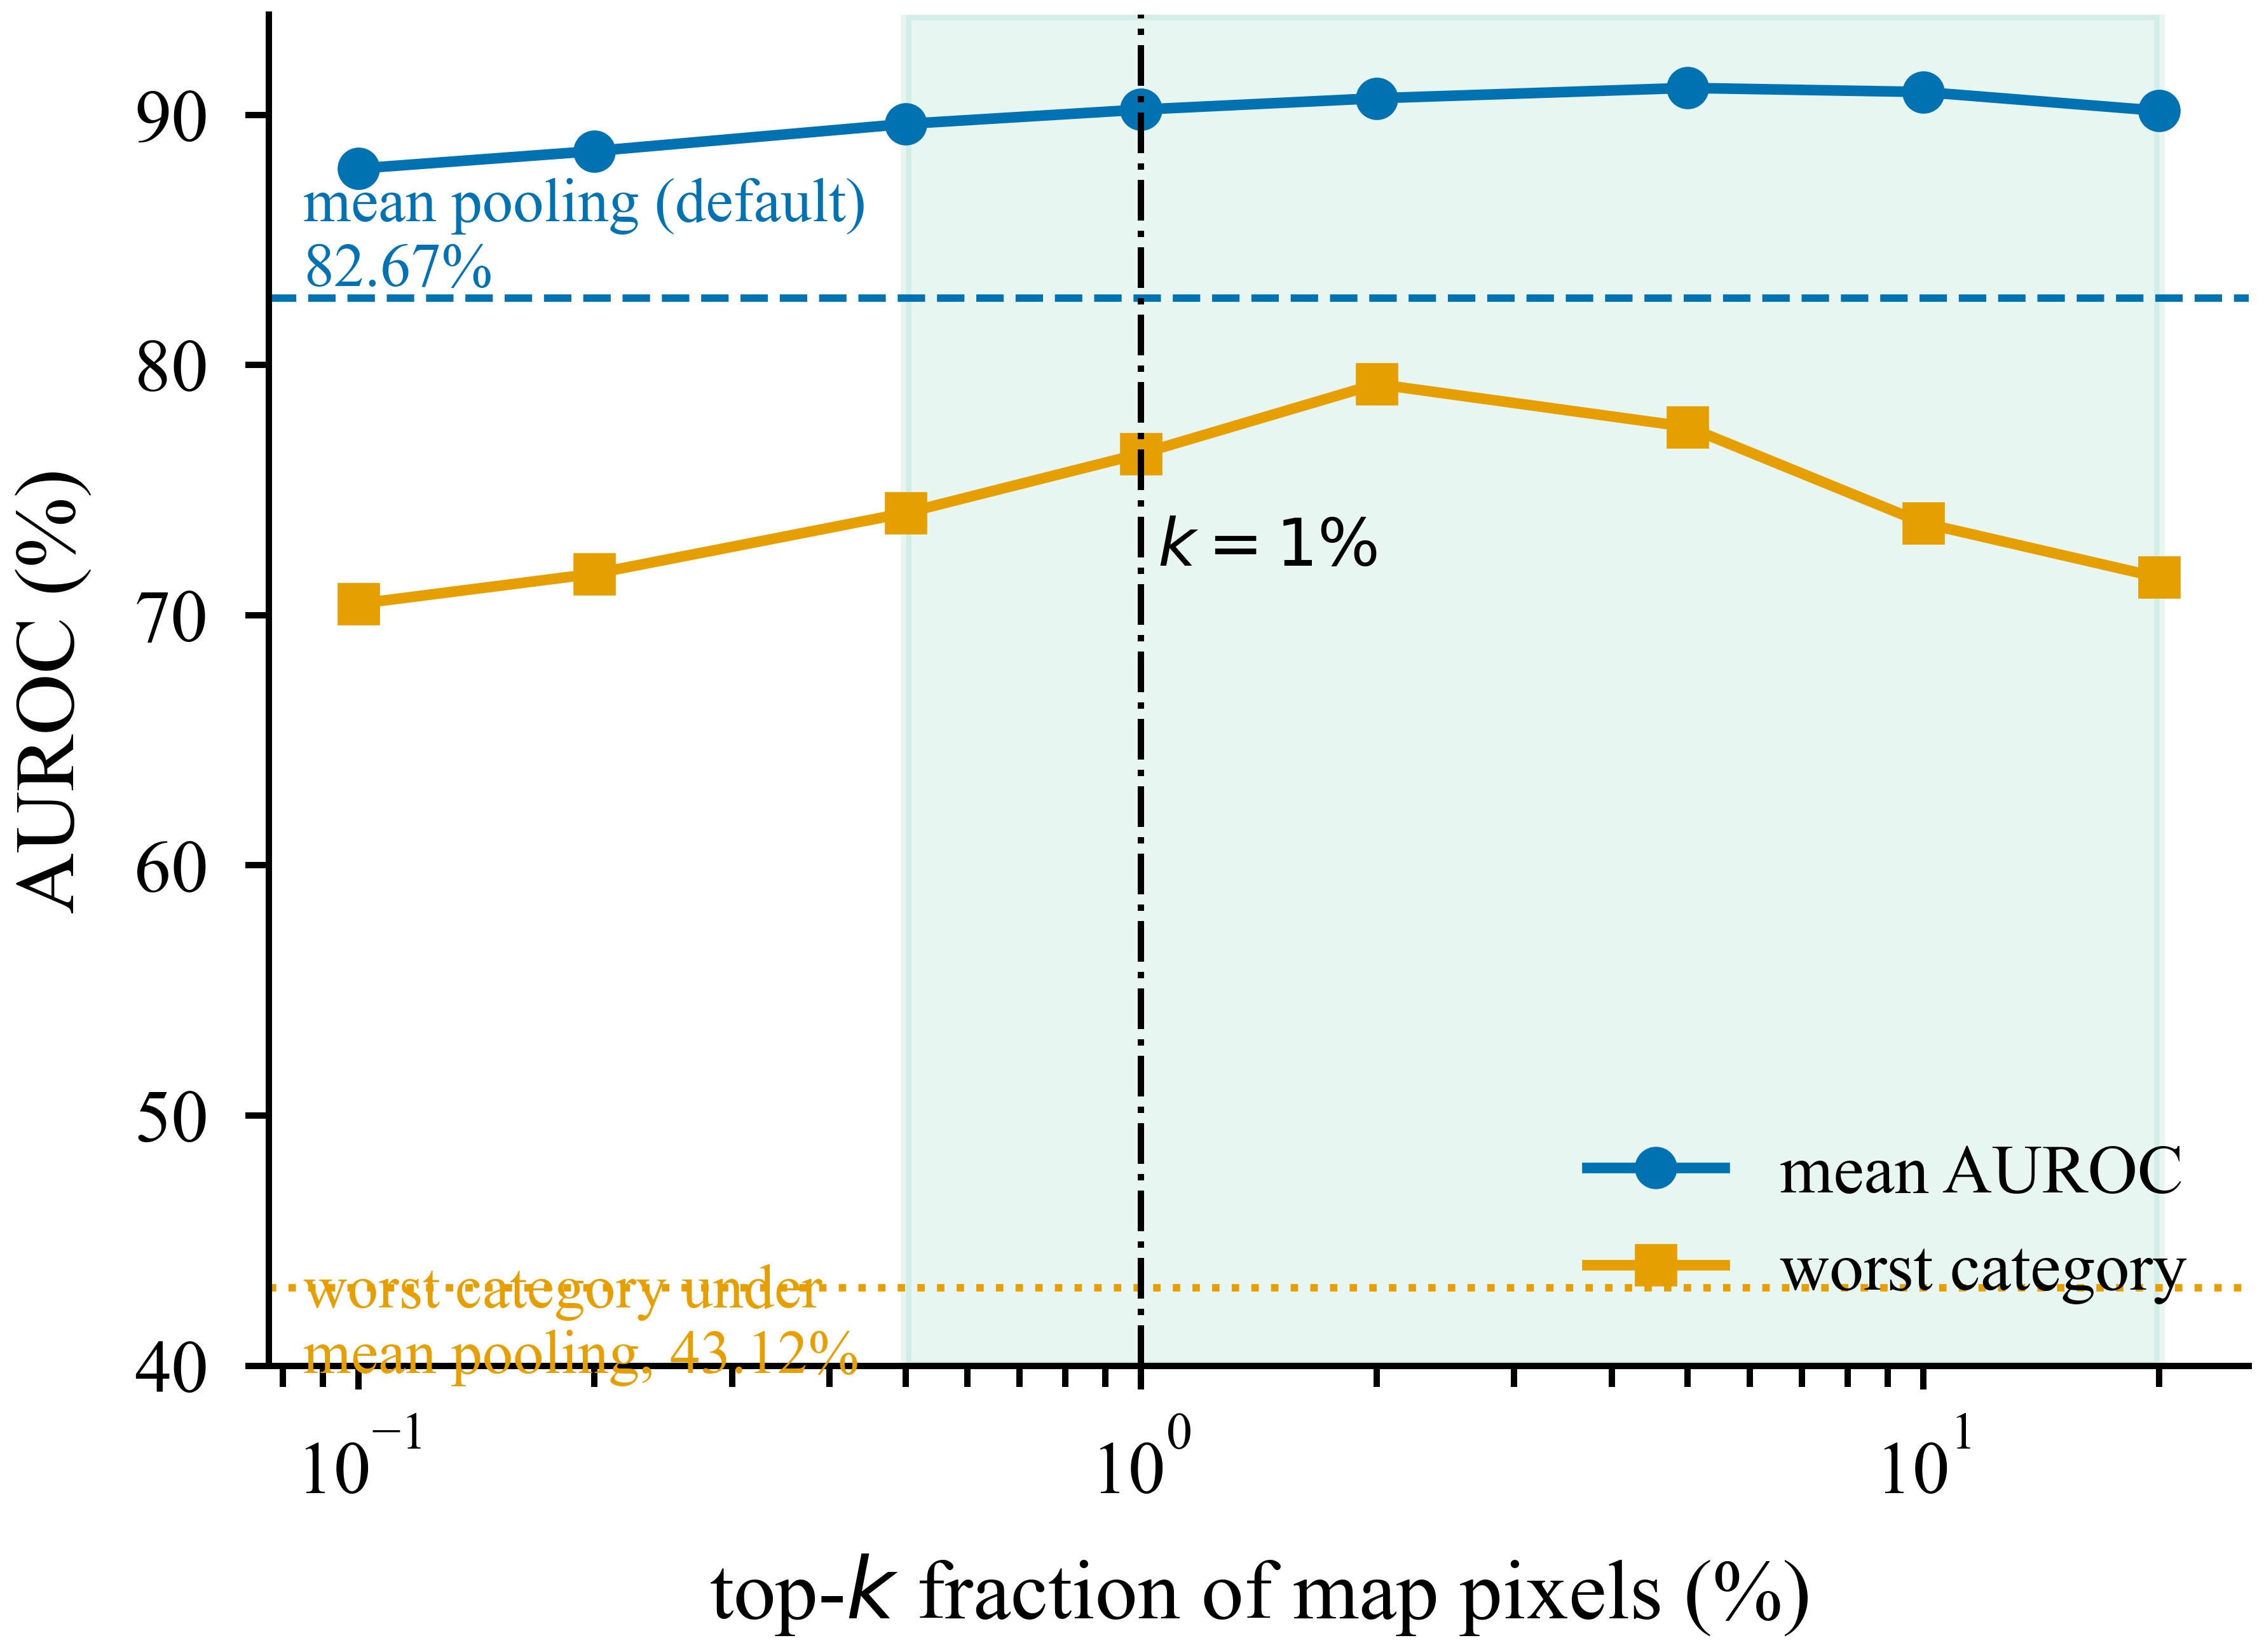
\includegraphics[width=\linewidth]{figures_v2/fig5_topk_sensitivity.png}
\caption{Sensitivity of the pooling gain to the top-$k$ fraction. The effect is a
broad plateau, not a spike: every $k$ between $0.5\%$ and $20\%$ recovers $7$ to
$8.4$ points of mean AUROC relative to mean pooling, and the published choice of
$k = 1\%$ lies inside the plateau rather than on its edge. The worst category peaks
earlier, at $k = 2\%$.}
\label{fig:ksweep}
\end{figure}

\begin{table}[t]
\centering
\caption{Sensitivity of the pooling gain to the top-$k$ fraction, uniform weights,
15 categories, computed by a second evaluation script on the same seed-42 trained
models. Every row in this table shares those maps, so the comparison is internally
exact. The two scripts \emph{disagree per category} even though their 15-category
means agree: for the identical policy (\texttt{sum\_topk} in the first script,
\texttt{uniform|topk\_0.01} in the second) the two read $90.21\%$ both, but their
per-category values differ by a mean absolute $0.74$ points and up to $2.49$
points (\texttt{tile}: $85.79$ vs $88.28$), and the worst-category statistic ---
the stated rationale for the $k$ range recommended below --- differs by $1.91$
points (\texttt{pill}: $78.37$ vs $76.46$). The default policy reads $82.67\%$
here against $82.80\%$ in Table~\ref{tab:fusion}, a $0.13$-point aggregate
difference that is the same level at which the two implementations agree on this
pipeline. We keep both scripts in the release and quote the range rather than
select one, and we flag that the per-category and worst-category numbers in this
section should be read as implementation-dependent to about two points. Two more
such pairs, for completeness: max pooling reads $86.74\%$ here against $86.84\%$ in
Table~\ref{tab:fusion}, and the best weighted policy reads $90.65\%$ here against
$90.60\%$ there.}
\label{tab:ksweep}
\resizebox{\columnwidth}{!}{%
\begin{tabular}{lrrr}
\toprule
Reduction & Mean AUROC (\%) & Worst category (\%) & $\Delta$ vs.\ mean pooling \\
\midrule
mean over all pixels (default) & 82.67 & 43.12 & --- \\
\midrule
1 pixel ($=$ max)   & 86.74 & 68.52 & $+4.07$ \\
$k = 0.1\%$         & 87.86 & 70.46 & $+5.19$ \\
$k = 0.5\%$         & 89.64 & 74.09 & $+6.97$ \\
$k = 1\%$           & 90.21 & 76.46 & $+7.54$ \\
$k = 2\%$           & \textbf{90.66} & \textbf{79.24} & $+7.99$ \\
$k = 5\%$           & \textbf{91.08} & 77.53 & $+8.41$ \\
$k = 10\%$          & 90.92 & 73.68 & $+8.25$ \\
$k = 20\%$          & 90.17 & 71.51 & $+7.50$ \\
\bottomrule
\end{tabular}}

\end{table}

\runinhead{What the pipeline's own noise floor is.}
The default policy's mean AUROC has now been measured three times on this
pipeline: $82.80\%$ here, $82.40\%$ in the earlier manuscript (an independent
training run of the same configuration, protocol and seed), and $82.67\%$ by the
second evaluation script behind Table~\ref{tab:ksweep}. The three agree to within
$0.4$ points, and the two that share the same trained models --- the first and the
third --- to within $0.13$ points on the aggregate. We report this rather than
average it away, because it sets the scale against which the effects in this
section should be read: the pooling gain is $7.42$ points, an order of magnitude
larger than the $0.13$--$0.4$ point aggregate spread of repeated measurement of
the baseline. It also illustrates the paper's central point at a smaller scale:
two implementations of the same statistic on the same models agree to $0.13$ points
in their 15-category mean --- a quarter of the $0.5$-point margin the field
contests --- while disagreeing per category by up to $2.49$ points
(Table~\ref{tab:ksweep}). Repeating a measurement with a second script therefore
moves the aggregate by a negligible amount and the individual numbers by more than
the margin being contested, which is itself an argument for reporting the
resolution of a design alongside its results. The per-category oracle, by
contrast, is an upper bound that requires anomaly labels and is reported to bound
what a selection procedure could achieve, not as an attainable number.

\runinhead{Catastrophic failures are a scoring artefact.}
The mean column of Table~\ref{tab:fusion} understates the practical importance of
the pooling choice, because the default policy does not merely lose accuracy on
average --- it fails catastrophically on specific categories. Under top-$k$
pooling the worst category rises from $42.22\%$ to $78.37\%$, and under the
per-category oracle to $84.67\%$. The clearest case is \texttt{screw}, where the
default policy scores $42.22\%$, below random guessing, while the same trained
model scores $84.01\%$ under top-$k$ pooling and $87.76\%$ under the best
per-category policy --- a gain of $41.8$ and $45.5$ points respectively. This
deserves emphasis because the manuscript attributes the \texttt{screw} failure to
a property of the detection paradigm and devotes a section to it; the failure is
produced by the reduction step. Averaging the discrepancy map over all pixels
destroys the signal whenever a defect occupies a small fraction of the image,
because the few genuinely anomalous pixels are diluted by the vast majority of
normal ones. \texttt{screw} consists largely of thin, localised thread defects,
exactly the regime in which a mean over the map is guaranteed to lose. The same
mechanism drives the other large top-$k$ gains: \texttt{metal\_nut} $+19.65$,
\texttt{grid} $+18.71$, \texttt{toothbrush} $+13.61$, \texttt{carpet} $+13.44$ and
\texttt{capsule} $+11.61$ points. Under per-category selection the largest
additional gains are \texttt{grid} $+27.90$, \texttt{carpet} $+21.55$ and
\texttt{metal\_nut} $+21.41$ points over the default. The pooling choice is
therefore not a refinement of a working method: it is the difference between a
detector that fails below chance on a standard benchmark category and one that
works on it, and it requires no retraining at all.

\runinhead{Scope of the pooling result.}
The comparison above is measured on one backbone family: the detectors carrying
the 82 policies are EfficientNet-B0 students
(Section~\ref{subsec:policy_results}), and we have not repeated the sweep across
the other thirteen backbones of the search space. The mechanism we identify --- a
mean over the map diluting small, localised defects --- is a property of the
reduction rather than of the network, and the per-category pattern (large gains on
\texttt{screw}, \texttt{grid}, \texttt{metal\_nut}; small losses on
\texttt{cable}, \texttt{pill}) is consistent with that reading, but we state
plainly that the sweep establishes the effect \emph{on this detector}, not across
architectures. Extending it to the other backbones is the most direct way to test
the mechanism, and it is future work rather than a claim of this paper.

It is also not the case that top-$k$ pooling dominates the mean everywhere. It
helps strongly on the six categories just listed, but it is slightly worse on
\texttt{transistor} ($-2.00$), \texttt{zipper} ($-3.02$), \texttt{tile}
($-4.62$), \texttt{pill} ($-4.80$) and \texttt{cable} ($-5.06$) points, on the
same trained models. The two poolings therefore respond to different defect
statistics, which is why per-category selection adds a further $3.5$ points on
top of the uniform top-$k$.

\subsection{Can the Policy Be Chosen Without Labels?}
\label{subsec:label_free}

The per-category oracle is not available in deployment, since it uses anomaly
labels. The practical question is whether $(\mathbf{w},\rho)$ can be selected
from normal data alone, which would make the gain available without ever using an anomaly label.

\runinhead{Normal-distribution criteria fail.}
A natural first attempt is to choose the policy under which normal training images
look most tightly clustered, or whose score distribution has the lightest tail. We
tested six such criteria on a held-out portion of the normal training data, for a
fixed model and its own held-out split; the default and oracle figures quoted in
this paragraph are that experiment's own ($82.39\%$ and $93.39\%$ on its split, on
a subset of the 82-policy grid), so they are not directly comparable with the
$82.80\%$/$93.72\%$ of Table~\ref{tab:fusion}, which uses the full training set
and the full grid. All six do worse than the default: the best
reaches $82.28\%$ against a default of $82.39\%$ ($-0.12$ points) and the worst
$81.12\%$ ($-1.28$ points), while the oracle over the same policies is $93.39\%$;
the criteria select the oracle policy in only 1--2 of 15 categories. The reason is
structural. Top-$k$ pooling deliberately amplifies the upper tail of the
discrepancy map, and on a normal image this tail is noise, so top-$k$ makes normal
data look \emph{less} well behaved, not more. Criterion and objective are therefore
anti-correlated: the property we would like a clean image to have is not the
property that makes a defective image detectable. Tightness of the normal
distribution is the wrong proxy, and no amount of tuning fixes a proxy measured on
the wrong side of the problem. The failure is one of criterion rather than of
estimation, so we replace it with a discriminative one.

\subsection{Discriminative Selection from Synthetic Anomalies}
\label{subsec:pseudo_results}

Held-out normal images are perturbed with synthetic anomalies---the device used
by DRAEM-style synthesis~\cite{zavrtanik2021draem}---and we select the policy
that best separates the perturbed images from their clean originals. Three
families of perturbation are used (smoothed blobs, thin oriented scratches, and
rectangular cuts), each with a per-image randomised strength, five seeds per
family, giving fifteen perturbed variants of the holdout set. Selection maximises
the area under the ROC curve between clean and perturbed holdout images. Only
\texttt{train/good} images are ever touched, so the procedure never sees a real
defect; and because it operates on a trained detector, adopting its output
requires no retraining.

Table~\ref{tab:pseudo} reports the outcome over all 15 categories and three
training seeds, and Figure~\ref{fig:label_free} the per-category detail.

\begin{table}[t]
\centering
\caption{Label-free selection of the scoring policy on 15 MVTec-AD categories,
from 111 candidate policies, repeated on three independently trained students.
Every row is measured on the same trained models within a column; no row above
the oracle requires a real anomaly label. Columns are individual seeds, because
they do not agree (see the text).}
\label{tab:pseudo}
\resizebox{\columnwidth}{!}{%
\begin{tabular}{lrrrr}
\toprule
Selection rule & Seed 42 & Seed 43 & Seed 44 & Mean \\
\midrule
default policy (\texttt{mean}, uniform) & 81.62 & 81.90 & 80.98 & 81.50 \\
\midrule
\emph{fixed} $\rho = \text{top-}k$, no selection (baseline) & \textbf{88.90} & \textbf{89.44} & \textbf{88.62} & \textbf{88.99} \\
\midrule
pseudo-anomaly separation, best policy & 89.99 & 89.96 & 85.81 & 88.59 \\
pseudo-anomaly separation, top-5 ensemble & 89.96 & 90.03 & 86.08 & 88.69 \\
pseudo-anomaly separation, top-10 ensemble & 89.70 & 89.98 & 86.25 & 88.64 \\
pseudo-anomaly separation, top-20 ensemble & 89.34 & 89.72 & 87.28 & 88.78 \\
\midrule
per-category oracle (uses labels; upper bound) & 93.19 & 93.36 & 92.90 & 93.15 \\
oracle top-5 ensemble (upper bound) & 93.81 & 93.52 & 93.12 & 93.48 \\
\bottomrule
\end{tabular}}

\end{table}

The rule that carries the gain is the pooling, not the selection. On the same
models and the same split, simply fixing top-$k$ pooling --- which needs no
criterion, no pseudo-anomalies and no selection step --- reaches $88.99\%$ on
average against $81.50\%$ for the default and $88.59\%$--$88.78\%$ for the four
pseudo-anomaly rules. The pseudo-anomaly criterion therefore does not beat the
fixed convention on average; it is a refinement whose own contribution is
$-0.40$ points, and its four variants all land in a $0.2$-point band that lies
\emph{below} the fixed convention rather than around it.

The procedure at its best policy returns $89.99\%$ on seed 42, $89.96\%$ on seed
43 and $85.81\%$ on seed 44, against the table's default row of $81.62$, $81.90$
and $80.98\%$ --- a mean gain of $\mathbf{+7.09}$ points over the default, and
$\mathbf{61\%}$ of the $+11.65$ points that per-category oracle selection would
have delivered on the same models.

\runinhead{But most of that gain is not the criterion's.}
Reporting the gain against the default policy alone would overstate the method,
and we therefore decompose it. The $61\%$ figure answers ``how much of the oracle
gap does the label-free procedure close?'', but it does not answer ``how much of
that does the \emph{criterion} contribute?'', and the two questions have very
different answers. The decomposition here is computed on this subsection's 70/30
split, so its fixed-top-$k$ gain ($+7.49$) is not the full-test-set figure
($+7.42$ on seed 42, $+7.78$ to $+8.07$ on the two later seeds) quoted in
Section~\ref{subsec:policy_results}; the two differ because the split does, and we
report both rather than translate one into the other. On the same 70/30 split and
the same trained students, replacing
the default with a \emph{fixed} top-$k$ policy --- that is, adopting the pooling
recommendation of Section~\ref{subsec:policy_results} and choosing no weights at
all, with no selection and no pseudo-anomaly data --- already reaches
$\mathbf{88.90\%}$ on seed 42, against $81.62\%$ for the default and $89.99\%$ for
the full procedure. Across the three seeds the fixed top-$k$ convention gains
$+7.28$, $+7.54$ and $+7.64$ points (mean $\mathbf{+7.49}$), while the
pseudo-anomaly criterion adds a further $+1.10$, $+0.52$ and $\mathbf{-2.82}$
points over that fixed convention (mean $\mathbf{-0.40}$). In other words, of the
$+7.09$ points attributed above to the label-free procedure, roughly $+7.49$ comes
from the plain decision to pool by top-$k$ rather than by the mean, and the
criterion's own contribution averages slightly \emph{below zero}: on two of three
seeds it is a small positive refinement, and on the third it is worse than simply
fixing $k$. We report this rather than let the larger number stand on its own,
because the honest reading of the evidence is that the useful, label-free
recommendation of this paper is \emph{the pooling}, and that the selection
criterion is an unproven refinement of it. The decomposition is released as
\texttt{pseudo\_select/baseline\_decomposition.py} and its JSON output.

This reading is reinforced by the control that filtering degenerate trials does not
rescue the criterion (Section~\ref{subsec:search_vs_random}), and by the fact that
the criterion's three-seed spread ($+1.10$ to $-2.82$ over the fixed convention) is
itself larger than its mean effect. The comparison is
within-model throughout, so the $+7.49$ is not a split artefact: it is the
pooling change measured on the same students.

The three seeds are worth reporting
individually because they do not agree: the gain over the default is $+8.37$,
$+8.07$ and $+4.83$
points on seeds 42, 43 and 44. The oracle gap is nearly constant across seeds
($11.46$--$11.92$), so the variability lies in the criterion rather than in what
is available to be recovered. This is the lesson of Section~\ref{subsec:resolvability}
at a smaller scale: a three-seed estimate of an effect this size is a range, not a
number, and a single-seed report of the label-free gain would have claimed $8.4$
points where the honest three-seed figure is $7.1$.

Two features of the procedure are stable even though its headline gain is not.
The pseudo criterion ranks policies by their true AUROC at a mean Spearman
$\rho = 0.53$ in \emph{every} seed ($0.529$--$0.536$): the ordering it learns is
reproducible, while the policy at the top of that ordering is not. And the
criterion selects the per-category oracle policy in only one of the forty-five
category-seed cells, yet still attains $88.59\%$ on average --- it does not need
to identify the optimum, only to move near-optimal policies to the front.
Ensembling the top five policies matches the single choice on average ($88.69$
against $88.59$) and is better in the weakest seed ($86.08$ against $85.81$), so
it is the safer default for a criterion with this much seed variance. Averaging
over more seeds and perturbation families is the obvious way to tighten it, and
we leave that to future work.

The comparison in Table~\ref{tab:pseudo} is measured on a student trained on 70\%
\begin{figure}[t]
\centering
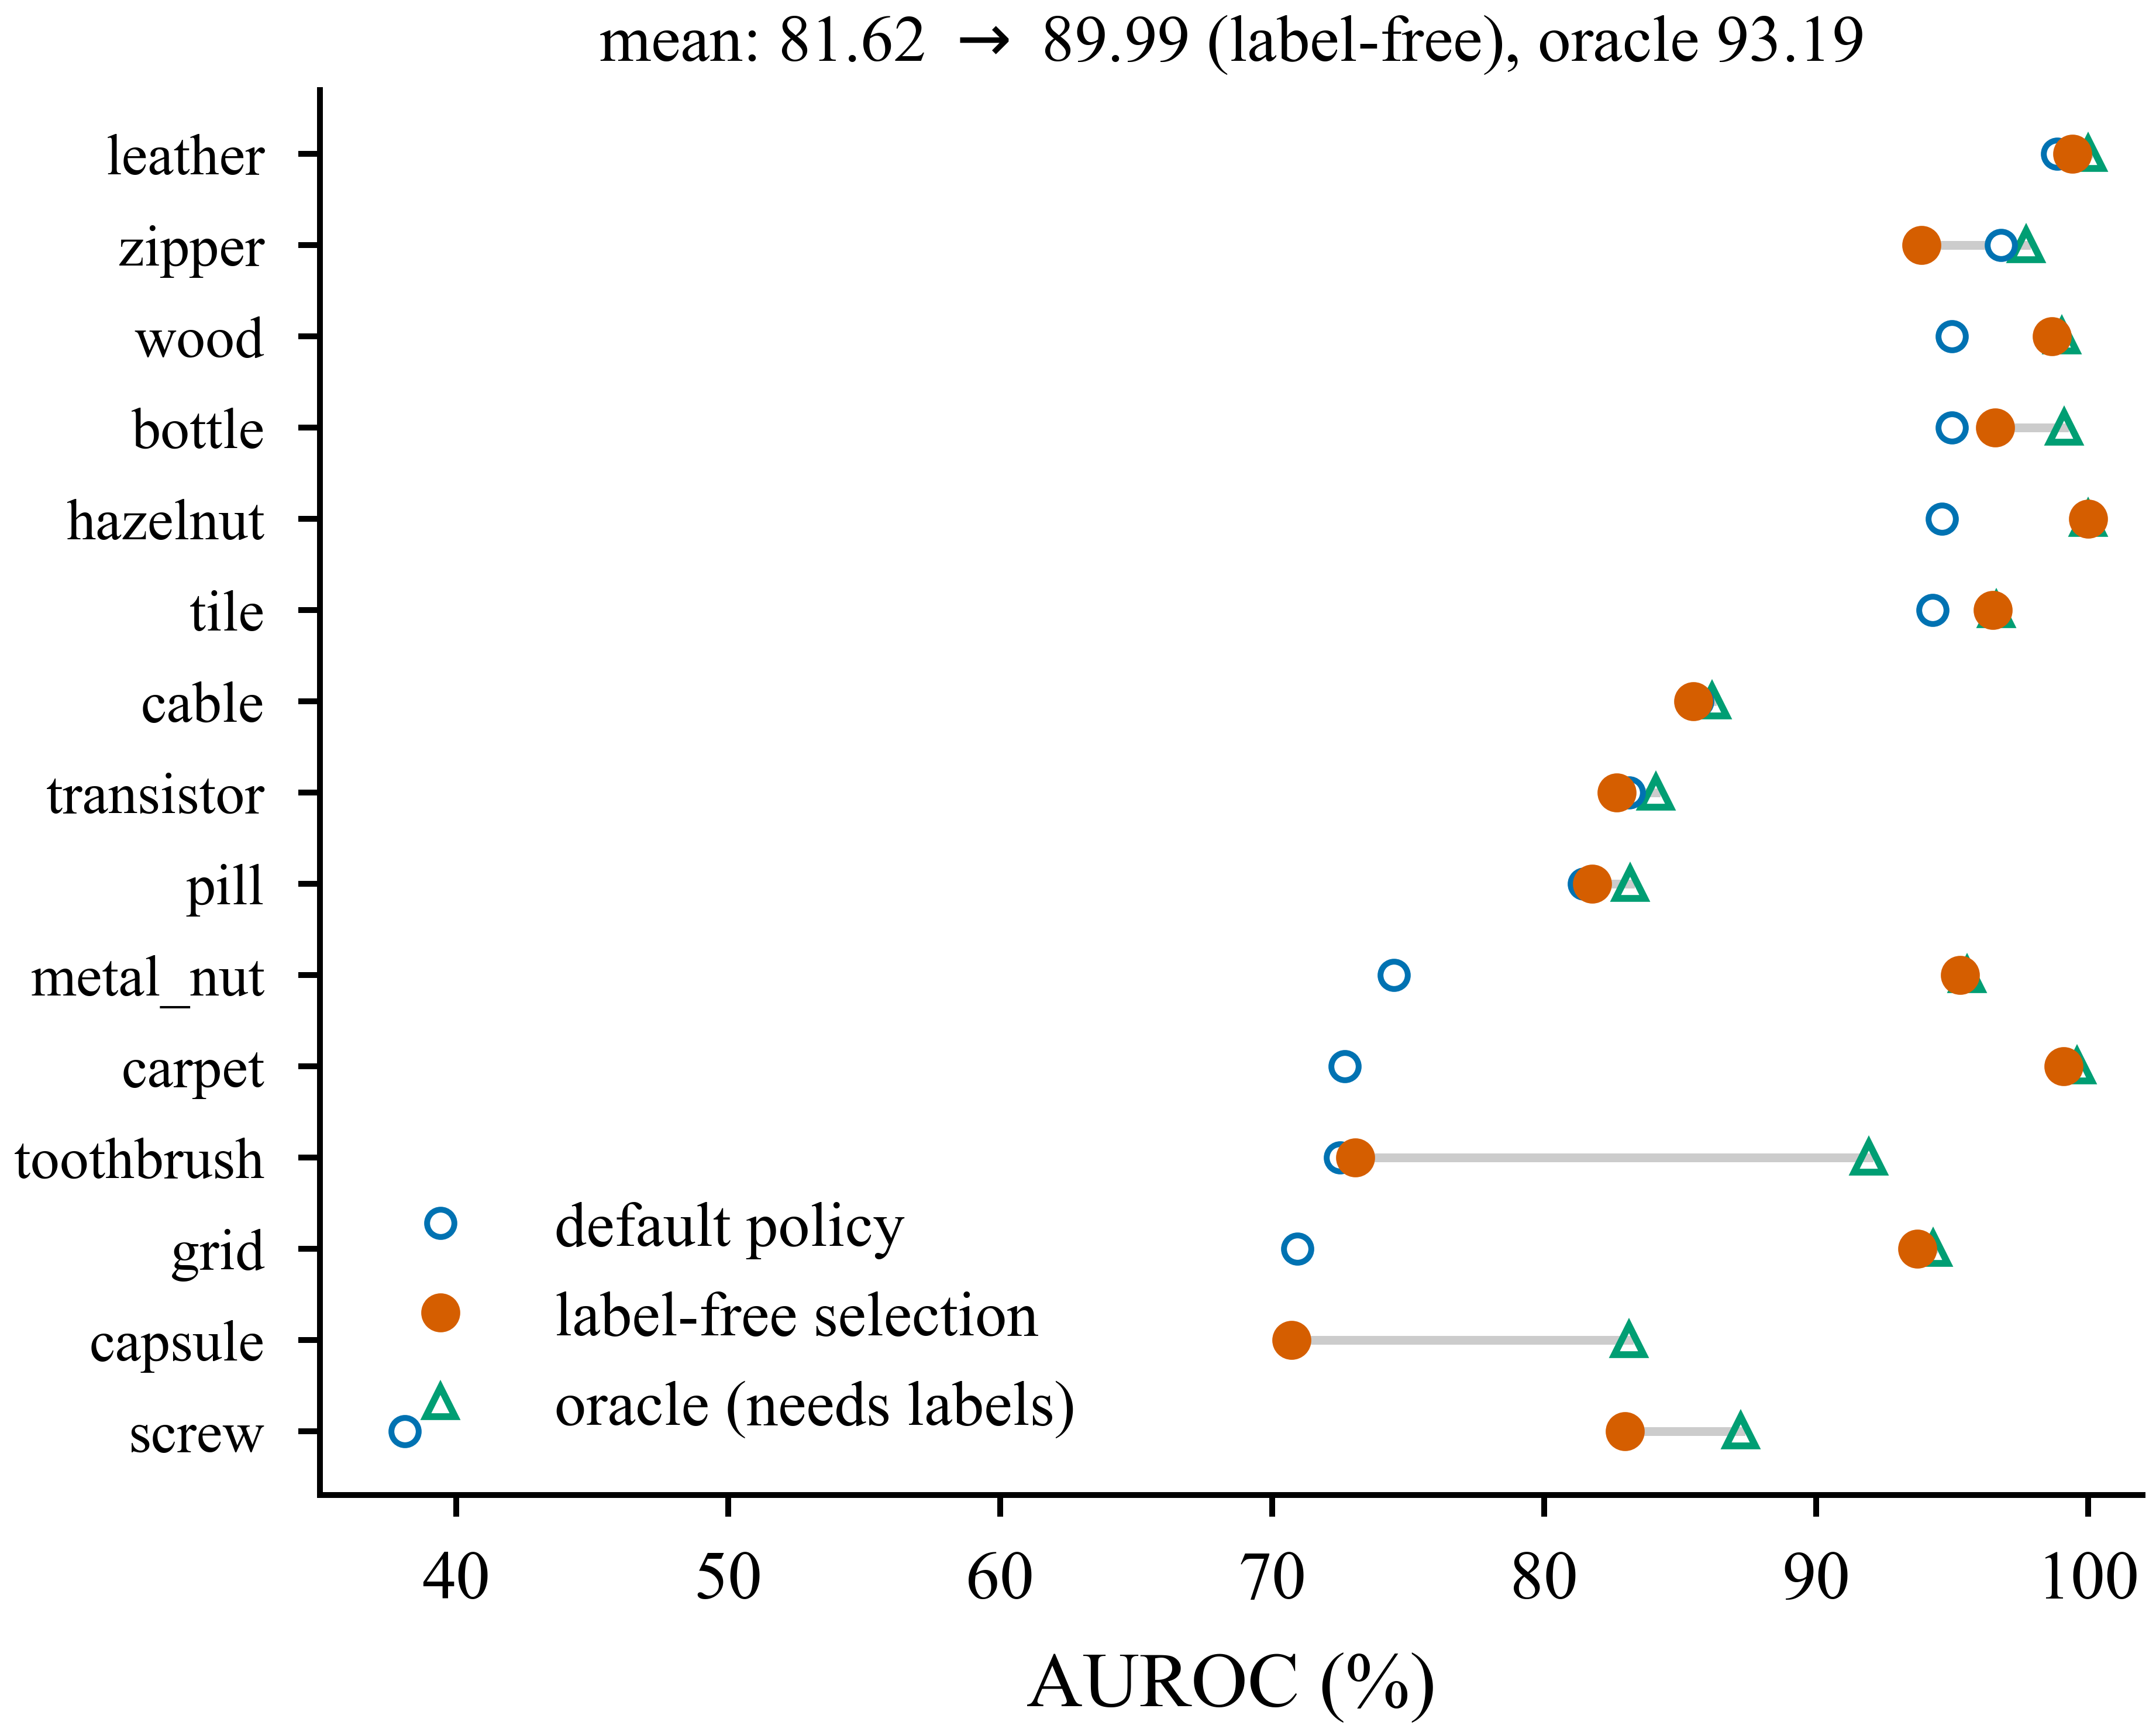
\includegraphics[width=\linewidth]{figures_v2/fig6_label_free_selection.png}
\caption{Label-free selection per category (seed 42). Hollow markers are the
published default policy, filled markers the policy chosen from synthetic
pseudo-anomalies without any anomaly label, and triangles the per-category oracle.
The label-free procedure recovers most of the available gap, and most of it on the
categories where the default policy fails badly (\texttt{screw}, \texttt{grid}).}
\label{fig:label_free}
\end{figure}

of the normal training images, with the remaining 30\% held out for selection
(the seed-42 default row is therefore $81.62\%$ rather than the $82.80\%$ of
Table~\ref{tab:fusion}, which uses the full training set). The gain is a
within-model comparison and is not inflated by the split; absolute numbers,
however, should be read with the split in mind.

\runinhead{Why the discriminative criterion works where the distributional one
fails.} The two criteria differ in what they ask of a clean image. The
distributional criterion asks that clean images look homogeneous, which top-$k$
pooling actively defeats. The discriminative criterion asks only that the policy
separate perturbed from clean --- the same question the detector is ultimately
asked at test time, posed on synthetic defects. It is a weaker and better-aimed
question, and it is answerable from normal data alone. Its own variance is the
open problem, not its direction.

% ============================================================================
% DRAFT v2 -- Section 6: Honest positioning
% Published values are as reported by the original authors (not re-run); the
% controlled comparison is our own (proxy_diag/phaseB_truth.json, 210 detectors).
% ============================================================================

\section{Discussion: Where This Pipeline Stands}
\label{sec:positioning}

This paper reports a diagnostic study, not a new state-of-the-art detector, and it
is therefore necessary to state plainly where the pipeline of
Section~\ref{sec:method} stands. Two comparisons are relevant. As \emph{reported by
the original authors}, image-level AUROC on MVTec-AD runs from $78.0\%$
(AutoEncoder) and $85.0\%$ (VAE)~\cite{bergmann2018improving} through $95.6\%$
(STPM)~\cite{wang2021stpm}, $96.0\%$ (SPADE)~\cite{cohen2020spade}, $97.9\%$
(PaDiM)~\cite{defard2021padim}, $98.5\%$
(reverse distillation)~\cite{deng2022reverse}, $99.1\%$
(PatchCore~\cite{roth2022patchcore}, EfficientAD~\cite{batzner2024efficientad}) and
$99.3$--$99.6\%$
(CFA~\cite{lee2022cfa}, FastFlow~\cite{yu2021fastflow},
SimpleNet~\cite{liu2023simplenet}, Dinomaly~\cite{guo2025dinomaly}). FastFlow
reports $99.4\%$. These numbers were not re-run here and their protocols are not
identical to ours, so they are for orientation only. Two of them, SPADE and
FastFlow, are preprints that were never published at a venue; they are included
because they are standard baselines in this literature, and their preprint status
is declared here rather than left implicit. The second comparison,
Table~\ref{tab:controlled}, is our own, in which all 14 backbones of the search
space were trained under one protocol on all 15 categories.

\begin{table}[t]
\centering
\caption{Controlled comparison: every backbone of the search space trained on
every MVTec-AD category under an identical protocol (500 epochs, batch size 64,
seed 42, ResNet-18 teacher, reverse distillation; 210 detectors). Deployed size is
the student encoder plus decoder. The manuscript's selected architecture is marked
with~$\dagger$. Mean AUROC and Rank are single-seed (seed 42) and should be read
with the resolution of Section~\ref{subsec:resolvability} in mind: \emph{every}
adjacent
rank differs by less than the $2.98$-point minimum detectable difference (the
largest adjacent gap is $0.75$ points), and only non-adjacent extremes --- for
instance rank $1$ against rank $13$, a gap of $3.23$ points --- exceed it. The
ordering is therefore resolved only at its extremes and unresolved across most of
its length. Six of the fourteen backbones were replicated at two further seeds; among
those six the ordering is \emph{identical} in all three seeds
(\texttt{resnet18} $>$ \texttt{efficientnet\_b0} $>$
\texttt{mobilenetv3\_small\_100} $>$ ViT-Tiny $>$ ConvNeXtV2-Tiny $>$
Swin-Tiny, maximum rank movement $0$), which is the evidence that the axis is
real but too small to be ranked by a single-seed comparison of the other eight.}
\label{tab:controlled}
\resizebox{\columnwidth}{!}{%
\begin{tabular}{lrrr}
\toprule
Backbone & Student (M) & Mean AUROC (\%) & Rank \\
\midrule
ResNet-18        & 13.04 & \textbf{83.34} & 1 \\
ResNet-34        & 23.15 & 82.99 & 2 \\
ResNet-50        & 25.77 & 82.75 & 3 \\
MobileOne-S0     &  6.27 & 82.58 & 4 \\
EfficientNet-B0$^\dagger$ & 5.41 & 82.47 & 5 \\
DeiT-Tiny        &  7.31 & 82.03 & 6 \\
MobileNetV3-Small & 2.81 & 81.85 & 7 \\
ViT-Tiny         &  7.31 & 81.51 & 8 \\
ConvNeXt-Small   & 51.39 & 81.43 & 9 \\
ConvNeXtV2-Tiny  & 29.80 & 81.35 & 10 \\
ConvNeXt-Tiny    & 29.75 & 80.91 & 11 \\
EfficientNet-B1  &  7.92 & 80.43 & 12 \\
Swin-Tiny        & 29.26 & 80.11 & 13 \\
ConvNeXtV2-Base  & 89.69 & 79.36 & 14 \\
\bottomrule
\end{tabular}}

\end{table}

The pipeline described in this paper reaches $82.47\%$ mean AUROC on MVTec-AD with
the architecture the search selected, \texttt{efficientnet\_b0} (5.41M parameters),
against reported values of $95.6\%$--$99.6\%$ for the established detectors. We
therefore do not claim a competitive operating point: the gap to the strongest
published single-class detectors is $17.1$ points, and we report it
rather than obscure it. We can also name at least one candidate cause. The
deployed detector uses an ImageNet-1k ResNet-18 as its frozen teacher
(Section~\ref{subsec:teacher}), whereas reverse distillation as published
pre-trains the teacher on the normal images of the target category; the same code
path also fixes the student bottleneck at a width the search cannot change. We do
not claim that these account for the whole gap, and we have not run the
teacher-adapted variant, so the attribution is a hypothesis rather than a result.
A second caveat is that the harness itself was not validated against a published
reverse-distillation configuration: we did not reproduce a reference RD number
inside our code path, so the $17.1$-point gap could in principle contain a
harness-level difference (for instance the batch-norm behaviour of the largest
backbones, which are trained with gradient accumulation and a smaller micro-batch;
Section~\ref{subsec:implementation}) on top of the teacher choice. We report this
rather than present the comparison as exact, and we note that it does not affect
the paper's diagnostic claims, which are all within-harness. Nor is the gap
explained by the parameter budget:
Section~\ref{subsec:capacity_null} varies the deployed size over a $9.2\times$
range across five capacity bands and finds no statistically resolvable effect, and
across the full space of Table~\ref{tab:controlled} the deployed size spans
$32\times$ while the backbone accounts for $0.54\%$ of the variance. One caveat
applies to the reported values: they come from implementations, augmentation
policies and training schedules that differ from ours, so the comparison is
indicative rather than exact. Table~\ref{tab:controlled} is the within-study
comparison on which the analysis in Section~\ref{sec:diagnosis} rests; it was
produced by the same code path, on the same data split, with one variable, the
backbone, changed at a time.

Two things are worth taking from Table~\ref{tab:controlled} in their own right.
It is, to our knowledge, the first comparison of a full anomaly-detection search
space under a single protocol, and as such it is a reusable resource: the ordering
it establishes is what makes the negative result in Section~\ref{sec:diagnosis}
measurable rather than anecdotal. And it shows that the search's output, at rank 5
of 14, is a reasonable but unremarkable choice from a space whose top eleven
candidates span $2.43$ points. The canonical headline number of this paper is the
$82.47\%$ mean AUROC of \texttt{efficientnet\_b0} on the fifteen categories, read
from the seed-42 truth matrix
(\texttt{proxy\_diag/phaseB\_truth.json}). An earlier, independently trained run of
the same configuration obtained $82.40\%$ on the same fifteen categories, a
difference of $0.07$ points. We report that agreement as a stability check and not
as confirmation: $0.07$ points is far below this paper's own $2.98$-point minimum
detectable difference, so the two numbers are simply \emph{consistent with} a
stable protocol, and the sentence cannot be made stronger without contradicting
Section~\ref{subsec:resolvability}. The search itself does \emph{not} reproduce as
closely;
Section~\ref{subsec:proxy_stability} documents why.

% ============================================================================
% DRAFT v2 -- Section 7: Conclusion
% Genre: benchmark / evaluation study.
% ============================================================================

\section{Conclusions}
\label{sec:conclusion}

This paper belongs to the class of studies that measure how a field evaluates
itself. Such studies do not add a detector; they establish what the field's
existing measurements are worth, and they are useful to the extent that the
answer changes how the next comparison is read. Our answer is that the standard
evaluation design for unsupervised anomaly detection cannot resolve the
differences the field reports, and that in the pipeline we instrumented the
design axis those comparisons are usually about contributes almost nothing.

The binding constraint is resolution. A two-way decomposition of the 210-detector
matrix we trained leaves a residual standard deviation of $3.30$ points, and the
run-to-run standard deviation of a single detector at a fixed (backbone,
category) is $1.96$ points over three seeds. Comparing two backbones across the
fifteen categories the benchmark provides is therefore a paired test whose minimum
detectable difference is $2.98$ points --- $75\%$ of the entire $3.98$-point
spread of the fourteen backbones, and six times the $0.5$-point margin that
separates PatchCore from the strongest results reported since. Resolving that
margin on a single category would take $240$ independent training runs per
backbone, or $532$ categories. This is a statement about the benchmark rather than
about our pipeline, and it bounds every architecture comparison made on it.

Within that constraint, the diagnosis of the architecture axis is unambiguous.
Two thirds of the search space is spent on a feature dimension that cannot reach
the deployed model, because the encoder that consumes it hard-codes a width while
the decoder honours the requested one. The search signal does not distinguish
architectures: it separates the eleven tight well-behaved backbones by $5.7\%$ of
its median, which is the same order as its own run-to-run noise, and it returns
exactly $0.0$ when a student diverges --- for two backbones in most trials, and
occasionally for any of them. And the quantity it is used to predict is dominated
something else entirely: architecture accounts for $0.54\%$ of the variance in
detection accuracy and the category for $95.32\%$
(Section~\ref{subsec:capacity_null}).

The interaction between the first two facts produces the result we did not
anticipate. Because the objective can silently return the optimum of its own
range, and the search minimises a single sample per candidate, the rule does not
select the best architecture but the one with the heaviest left tail --- which is
the one that failed. Twelve independent runs selected a configuration prone to
this collapse every single time, and the architectures they returned perform
\emph{worse} than uniform random selection, at the $1.2$th percentile of the
random distribution (Section~\ref{subsec:search_vs_random}). The four runs whose
results the manuscript originally reported chose a backbone that does not
collapse, which on this account was luck.

The constructive finding is where the accuracy actually is. The reduction that
turns a multi-scale discrepancy map into an image-level score is worth $+7.92$
points of mean AUROC across three training seeds --- an order of magnitude more
than the architecture --- and it is worth those points without retraining
anything. The default choice, an unweighted mean over all pixels, is not merely
suboptimal: it fails below chance on \texttt{screw}, and top-$k$ pooling repairs
that failure to $84\%$. The gain is robust across two orders of magnitude in $k$
(Section~\ref{sec:leverage}). And the reduction can be chosen without any anomaly
label, by perturbing held-out normal images with synthetic defects and selecting
the policy that best separates them from the clean ones: averaged over three
training seeds this recovers $61\%$ of the oracle gap, though the seeds range from
$41\%$ to $72\%$, so it is a direction rather than a settled number.

Three limitations bound these claims. The diagnosis is established on MVTec-AD,
with one teacher, one detector family and one training protocol; whether the same
collapse appears in other pipelines is a question our evidence cannot settle,
though the mechanism --- a thresholded objective that can return its own optimum,
combined with a minimising selection rule --- is not specific to this codebase.
Our recommendation for the architecture axis is deliberately narrow: the backbone
effect is statistically detectable ($p = 0.039$) and merely two orders of
magnitude smaller than the category effect, so we do not conclude that
architecture does not matter, nor that NAS for anomaly detection is worthless in
principle. And the resolvability figure is conditional on this benchmark's fifteen
categories and this task's residual variance; it should be recomputed rather than
assumed for another benchmark or detector family --- which is exactly the
calculation a benchmark paper ought to publish, and which here decides the
question.

Two things follow for practice. A search whose objective can silently return the
optimum of its own range must filter degenerate evaluations before minimising, and
should report the distribution of its per-configuration scores rather than a
single minimum. And any deployed reverse-distillation detector currently scoring
images by the mean over its discrepancy map can be re-scored, on the models it
already has, with a $k$ of two percent, and expect to gain several points of
accuracy and to stop failing below chance on the categories that currently defeat
it. Neither of those requires convincing anyone that a new architecture is better,
which is convenient, because on this benchmark that cannot be shown.


%%=============================================================================%% Back matter
\backmatter

\bmhead{Acknowledgements}

This work was supported by the Guangxi Natural Science Foundation (Grant No. 2025GXNSFHA069076) and the Guangxi University of Science and Technology Doctoral Fund (Grant Nos. 26Z15, 26Z25).

\section*{Statements and Declarations}

\begin{itemize}
\item \textbf{Funding}: This research was supported by the Guangxi Natural Science Foundation under Grant No. 2025GXNSFHA069076 (awarded to P.D.) and by the Guangxi University of Science and Technology Doctoral Fund under Grant Nos. 26Z15 (awarded to P.D.) and 26Z25 (awarded to H.L.). The funders had no role in the design of the study, in the collection, analysis or interpretation of data, or in the decision to publish.

\item \textbf{Competing interests}: The authors declare that they have no known competing financial interests or personal relationships that could have appeared to influence the work reported in this paper.

\item \textbf{Ethics approval and consent to participate; consent for publication; materials availability}: Not applicable. This study did not involve human participants or animals, and no new materials were generated.

\item \textbf{Data availability}: This work uses only the publicly available MVTec-AD benchmark~\cite{bergmann2021mvtec}; no new image data were generated. Every derived artefact is released together with the code (see below): the architecture-search logs, the per-configuration proxy evaluations, the 210-detector AUROC matrix, the per-run search records, the auxiliary benchmark harness, the synthetic-mechanism study, and the scripts that regenerate every table and figure. Each number reported in this paper can therefore be traced to the run that produced it.

\item \textbf{Code availability}: The complete source code and the raw experimental logs are publicly released at \url{https://github.com/fanta12138/kg-nas-diagnosis}, under a MIT licence. They comprise the pipeline under study, the diagnostic experiments (proxy repeatability, the truth matrix, the repeated searches), the synthetic reproduction of the degeneracy mechanism, the resolvability analysis, the benchmark harness, and the analysis scripts that produce every table and figure in this paper, together with a SHA-256 manifest of every released file.

\item \textbf{ORCID}: P.D. \url{https://orcid.org/0000-0002-2892-4251}. The remaining authors will supply their identifiers to the editorial office at submission.

\item \textbf{Author contributions}: All three authors are colleagues in the same school and jointly planned the study. Using the CRediT taxonomy:
\textbf{Conceptualization}, P.D.; \textbf{methodology}, P.D., H.L. and Y.Z.; \textbf{validation}, P.D.; \textbf{formal analysis}, P.D.; \textbf{writing---original draft preparation}, P.D.; \textbf{writing---review and editing}, H.L. and Y.Z.; \textbf{supervision}, P.D.; \textbf{project administration}, P.D.; \textbf{funding acquisition}, H.L. and P.D. All authors have read and agreed to the published version of the manuscript. P.D. is the corresponding author.

\item \textbf{Use of large language models}: An AI assistant (a large language model) was used substantially in this work. It wrote the code for the diagnostic experiments, the synthetic reproduction and the benchmark harness, executed those experiments, and produced the numerical results reported here; it also produced drafts of the manuscript text and the plotting code. No figure or table was generated by a generative model: each figure is a plot of recorded measurements produced by the released script, and each table transcribes the same recorded result files. The authors specified the research questions, directed the work, verified the reported results against the recorded experimental outputs, and take full responsibility for the content, the claims and their accuracy.
\end{itemize}

%%=============================================================================%% References
\bibliography{references}

\end{document}
